% REMEMBER: You must not plagiarise anything in your report. Be extremely careful.

\documentclass{l4proj}

    
%
% put any additional packages here
%

\begin{document}

%==============================================================================
%% METADATA
\title{Tangible 2-Factor Authentication\\ \Large{Designing and Investigating Authentication Objects for Daily Usage}}
\author{Mark Turner}
\date{January 26, 2022}
\maketitle

%==============================================================================
%% ABSTRACT
\begin{abstract}
   ``Two-factor authentication is already a widely used and recommended method of securing one's data, however most of the preferred solutions tend to remain in the digital space.  This project investigated the usability of tangible, 3D-printed objects that made use of a conductive form of plastic to interact with a capacitive touch screen. This paper finds whether this type of authentication can compare to existing two-factor authentication solutions by performing a week-long field study culminating in a recorded interview, having developed model designs based on user feedback as well as creation of a mock authentication app for data collection. This paper finds that, compared with other two-factor methods, while T2FA is less usable currently with the lack of feedback being cited as a major problem, it shows great promise, with participant feedback indicating a high interest level in a more developed version. With further development in this area, this could become a widespread method of authentication with a good amount of re-usability without sacrificing account security as with repeated passwords.``

\end{abstract}

%==============================================================================

% EDUCATION REUSE CONSENT FORM
% If you consent to your project being shown to future students for educational purposes
% then insert your name and the date below to  sign the education use form that appears in the front of the document. 
% You must explicitly give consent if you wish to do so.
% If you sign, your project may be included in the Hall of Fame if it scores particularly highly.
%
% Please note that you are under no obligation to sign 
% this declaration, but doing so would help future students.
%
\def\consentname {Mark Turner} % your full name
\def\consentdate {26 January 2022} % the date you agree
%
\educationalconsent


%==============================================================================
\tableofcontents

%==============================================================================
%% Notes on formatting
%==============================================================================
% The first page, abstract and table of contents are numbered using Roman numerals and are not
% included in the page count. 
%
% From now on pages are numbered
% using Arabic numerals. Therefore, immediately after the first call to \chapter we need the call
% \pagenumbering{arabic} and this should be called once only in the document. 
%
% Do not alter the bibliography style.
%
% The first Chapter should then be on page 1. You are allowed 40 pages for a 40 credit project and 30 pages for a 
% 20 credit report. This includes everything numbered in Arabic numerals (excluding front matter) up
% to but excluding the appendices and bibliography.
%
% You must not alter text size (it is currently 10pt) or alter margins or spacing.
%
%
%==================================================================================================================================
%
% IMPORTANT
% The chapter headings here are **suggestions**. You don't have to follow this model if
% it doesn't fit your project. Every project should have an introduction and conclusion,
% however. 
%
%==================================================================================================================================
\chapter{Introduction}

% reset page numbering. Don't remove this!
\pagenumbering{arabic} 

With touchscreens becoming more ubiquitous and the devices using them requiring authentication more frequently, fast and simple methods have become the preferred way to access devices and accounts, with pins and patterns taking precedence over more secure 2-factor methods [\cite{colnago2018s}, \cite{reese2019usability}]. As such, the importance for a method of secure authentication that users will happily use has become greater over the years, as too many 2-factor methods are considered cumbersome and a waste of time by some users [\cite{10.1145/3503514}, \cite{das2018johnny}], by forcing them to jump back and forth between tabs and devices, waiting for codes to generate or requiring multiple additional devices that rely on network or battery. Something new is needed to solve these issues and improve the adoption of 2-factor authentication as a whole, allowing users to secure their account from malicious actors without sacrificing usability - a failing of contemporary methods. Even those 2FA methods developed that have been found to be more usable than passwords tend to leave users with some concerns affecting adoption rates [\cite{9152694}]. Tangible authentication offers a break from these problems by presenting more enjoyable method, as well as being more open to the addition of customisation [\cite{sherman2014user}].

This project presents Tangible 2-Factor Authentication (T2FA), a simple method of 2-factor authentication using a physical, 3D-printed model and a capacitive touchscreen device to authenticate a user through ownership of the object and the knowledge of how to use it. The object, using an interaction space previously defined by \cite{marky20203d}, takes the form of a small, everyday object with touch points encoded in the model's structure made from a conductive plastic that interpret the user's interaction with the model and convey it onto their touchscreen device to authenticate. 

Previously, 3D printed objects have been shown to work in lab studies, however these studies have not used realistic dimensions, as a result, performance under daily usage is unclear. This work fills this gap by creating a group of models based on user feedback, with the three most suitable being selected for use in a long-form field study. This study aimed to specifically investigate the usability of the authentication method in this way by introducing it into potential users' daily routines. To facilitate this, an Android app was built for users to perform mock authentications with their assigned model during the study, as well as to collect data on their use.

This project saw a preliminary study carried out, with one participant selected for each of the models and asked to perform authentications throughout their day for a week and return to feedback on their experiences, results of which indicated that while the method proved to be less usable than other contemporary 2-factor methods with data indicating a lower average SUS score, the participants were each eager to welcome tangible two-factor authentication in the future as an alternative to other contemporary methods.

Hence, while it certainly requires further development to improve on consistency of interaction reads and better methods of tracking ownership, T2FA shows great promise in becoming a new method of two-factor authentication, offering a break from purely digital methods with a more fun and concrete interaction which this paper found to be important to users, allowing for users to take security into their own hands.
 \newpage
The remainder of this paper is structured as follows: 
\begin{itemize}
    \item Chapter 2 introduces the background information required to fully understand this project
    \item Chapter 3 outlines previous work done in related areas that this work draws on
    \item Chapter 4 details the concept of the paper and what was carried out
    \item Chapter 5 outlines the evaluation methodology and obtained results from a usability study performed
    \item Chapter 6 is a discussion of the results found as well as potential implications of this work
    \item Chapter 7 concludes the work
    \item Chapter 8 gives acknowledgements to those that helped
\end{itemize}


%==================================================================================================================================
\chapter{Background}

To fully understand the work presented, relevant areas have been outlined to ensure a base level of knowledge. In particular, this section will discuss \textit{two-factor authentication in a general sense, 3D-Auth, 3D printing and object recognition}, and \textit{technical details}.

\section{Two-Factor Authentication}

Authentication can be performed through three different methods, or factors - these being knowledge, ownership and inherence. Passwords are the most widely used method of authentication, being knowledge based, however, these tend to have security issues surrounding their weak nature due to reuse or simplicity and in some cases how they are stored by service providers being vulnerable to attack [\cite{10.5555/3235838.3235860}, \cite{10.5555/3235866.3235877}], leading to less secure accounts. Two-factor authentication expands authentication further, adding another required check before verifying access, a widely used example of which are bank cards, which use a knowledge based pin and a personal card as an ownership check. In the case of T2FA, these two factors mirror the example given, with a knowledge and ownership factor.

\section{3D-Auth}

3D-Auth [\cite{marky20203d}] described the use of 3D printed models for tangible authentication, outlining different methods of interaction (such as touching a specific part of an object or assembling multiple models in a certain way) after performing a design study with experts from different areas. The paper built prototypes for each of these interaction types and assessed them in a lab study to find how usable and memorable the methods of interaction were. The prototypes were created using 3D printing of conductive and non-conductive materials designed in such a way that interactions could be read by a capacitive touch screen and validated using a smartphone app. Being prototypes, the models used in the study were bulky, with each object being large proving difficult to perform a user field study with, so this study hopes to improve on this, taking the interaction space that was defined and designing new models to assess the principle of this form of tangible authentication for daily use. 

\section{3D Printing and Object Recognition}

The models have been designed to utilise conductive (cPLA) and non-conductive (PLA) filament. The basic method of interaction when using the models involves placing the object onto the touchscreen, then performing an action. Each action requires that the user touch one or more specific parts of the object, with each of these parts containing conductive material. The touches performed on the object are transmitted by internally printed conductive PLA to the capacitive sensors on the touchscreen, activating the sensors in the same way a finger would. The touches read by the screen are then interpreted by the authentication program and translated into either a pass or fail. More simply, the model acts as a middleman between user and touchscreen, turning the user's actions with the model into a sort of pass code read by the screen, this is the knowledge factor. In addition to this, the models itself also contains a space for a 'footprint', that is, a unique series of points that would identify ownership of the model that is also read by the touchscreen - the ownership factor.

\section{Technical Details}

The models were each printed with a Prusa MK3 printer [\cite{prusaprinter}], with a multi-material unit attachment (MMU2.0) [\cite{prusammu}], allowing for multiple filaments to be loaded at a time when printing. This is how the internal 'wiring' was achieved. To ensure it was easy for users to find the touch points, as well as for aesthetic reasons, the non-conductive PLA was a different colour from the conductive - in the case of this study, the insulating PLA was red while the cPLA was black.

%==================================================================================================================================

\chapter{Related Work}

In this section, previous research contributions that this work builds upon will be discussed. In particular, there are 3 relevant areas of research for this project that are detailed: \textit{two-factor authentication, 3d printed interactive objects}, and \textit{tangible authentication.}

\section{Two-Factor Authentication}
 
 Many methods of authentication involving two factors have already been proposed, with some already in use by end-users on different platforms and services. Some utilise one-time passcodes which are transmitted to the user via email, SMS [\cite{5069395}], or in some cases generated by a physical token [\cite{duo}]. However, these often trade-off usability, resulting in low adoption rates when not mandatory due to the perceived hassle of using it - failings like SMS arriving too late come to mind. Additionally, research has been done proving the ineffectiveness of some methods of digital two-factor authentication, outlining various methods of attack exploiting them such as Trojans [\cite{dmitrienko2014security}] or phishing attacks [\cite{markert2019view}]. \\
 The reason behind low adoption rates has been investigated thoroughly. \cite{bonneau2012quest} defined eight usability criteria, and found that none of the contemporary schemes analysed met all of them fully, finding them as more secure but generally less usable than traditional passwords. Additionally, \cite{colnago2018s} found that, despite a usable design, some users are still put off and tend not to use two factor authentication due to bias from previous experience, suggesting social influence is important in ensuring adoption, and research done by \cite{dewitt2006aligning} showed that users valued the speed and ease with which tasks could be completed over security, indicating that the extra steps required by two-factor authentication itself tends to be cumbersome for users. For a two factor authentication method to be widely adopted, it must be fast, easy to use and even potentially different enough from those contemporary methods already employed that users with a bias against would be willing to use it. It could indeed be said that two factor authentication has an image problem, and new methods following the paradigm should consider a change in name.

\section{3D Printed Interactive Objects}

Regarding this project, the most relevant line of research involves some method of embedding conductive material into the object, whether through the use of a conductive spray on a completed object [\cite{10.1145/2556288.2557046}] or a conductive plastic embedded into printed models for various usages [\cite{10.1145/1979742.1979773}, \cite{10.1145/2207676.2208371}, \cite{schmitz2021itsy}, \cite{schmitz2018off}, \cite{marky20203d}, \cite{leigh2012simple}, \cite{kato20163d}] as in this project.\\
Another line of research has involved embedding sensors into 3D printed models to allow for interactivity. In particular, methods involving the use of capacitive [\cite{10.1145/2207676.2207743}] or acoustic [\cite{10.1145/2501988.2501989}] sensors to detect touch or sound, or through the use of accelerometers [\cite{10.1145/2559206.2581137}]. This allows for more complex interactions to be registered, however it also requires additional assembly and technical knowledge, creating more overhead which this project wished to avoid.\\
Other research has produced methods of fabricating interactive elements in other ways via digital pipelines, such as those involving optical elements [\cite{brockmeyer2013papillon}, \cite{willis2012printed}] or filling pipes with other media [\cite{savage2014series}], to create highly customizable interactive devices. In addition to this, materials have been used for the creation of flexible [\cite{schmitz2017flexibles}] or soft [\cite{peng2015layered}] objects, allowing for deformations as an interaction method.


\section{Tangible Authentication}

Multiple different approaches have been outlined in research for dealing with tangible authentication. One such method is TwistIn [\cite{leung2018twistin}], which utilises the sensing information in smart devices to detect simple twist gestures which are then co-analysed with the same information from the user's smart-watch to perform authentications with an accuracy of 95\%, however this method is limited for use only in small, handheld devices. \\
Another method is the Phone Lock system [\cite{bianchi2010phone}], which uses audio or haptic feedback to indicate to the user the PIN they require to authenticate, creating an interaction safe against shoulder surfing. The study performed found that the mean error rate was 7\% and average authentication time for 4 PIN authentication was 13.5 seconds, deeming the results very promising, and demonstrating that secure authentication methods need not sacrifice usability heavily.
Other devices utilise wearable tokens [\cite{chen2008tangible}] or RFID [\cite{klompmaker2012authenticated}] to verify the identity of users.


%==================================================================================================================================
\chapter{Concept}

In this section, the development of the project will be discussed, outlining the initial requirements decided upon, issues that were found, and the final designs used in the user field study.

\section{Initial Investigation}

The initial goal of the project was to investigate the long-term interactions between users and tangible objects for authentication, in particular, objects that follow the paradigm laid out by \cite{marky20203d}. Since the objects used in the lab study performed were prototypes simply demonstrating the methods of interaction, new objects would have to be made that followed the same method but took on a more desirable form for users. To that end, an existing online survey investigating the perceptions of this type of authentication among the general populace, as well as finding desirable traits that could be adapted for use in an 'alpha' version of this system of tangible two factor authentication served as a basis for this project.

\subsection{Survey Analysis Method}

To begin the analysis of the data set, it was initially filtered by four understanding questions, to ensure that participants read and comprehended the contents of the survey. This reduced the number of respondents to 88 valid responses. The relevant criteria investigated for this project were each open text questions, requiring manual investigation and categorisation. The method for categorisation of the responses will be outlined, and the tables created through the analysis can be found in Appendices Section \ref{sec:onlineana}.

In investigating the shapes of objects that were most desired, inductive categorisation was used to generalise answers. The results collected on Table \ref{tab:modshape} found that respondents most preferred a cube-shaped design, with other common responses being credit card-shaped and coin-shaped.

Additionally, the size most desired for these objects were collected. In cases where the respondent provided a range, the lower number was chosen, and all sizes were recorded as centimeters. In Table \ref{tab:modsize}, it can be seen most respondents fell in the range of 5 to 10 centimeters, but more generally, users clearly opt for smaller sizes, reasoning \textit{'[so] it is portable'} (P251) and \textit{'bigger than that is excessive'} (P286).

\section{Creation of Final Models and Authentication App}

Having obtained data on desirable qualities of such objects from the online survey analysis, prior to performing the field study two more areas would have to completed: creation of the objects to be assessed and creation of a mock authentication app. Due to the reliance both of these areas had on each other, it was decided that development should be done on them concurrently, to allow for problems to be diagnosed and dealt with quickly. Before this, however, the potential models had to be designed according to the findings.

\subsection{Iterative Design of the objects}

The process that was undertaken for designing the models began by choosing the eight most desired shapes discovered, with designs being sketched out for the following types of models: \textit{cube, circle/coin, credit card, square, animal, necklace pendant} and \textit{keyring}. These were chosen as they were the shapes found to be specified by multiple respondents in the analysis of the online survey, with 'phone case' being discarded from the list due to inability to plan for the size of phone participants will have, as well as 'wearable (ring)' due to the inability to plan for different participant ring sizes. Following this, multiple interaction methods were considered, initially the 'Augmentation' method was the only method immediately removed from consideration due to the requirement of external material being unfeasible for objects in the field study which should remain usable everywhere, as well as already being found to be the least usable method in the previous lab study.

The initial designs were created keeping in mind the existing constraints in place due to the 3D printing required. Each of the models was to be created with hard plastic, so no flexibility could be integrated into the designs. In addition, the models were to be designed as simply as possible, in an attempt to remove the need for any support structures during printing or extra alteration to the models after printing such as excessive sanding. Additionally, in the initial stages of design, the footprint was represented as a square touch point on some models which could be used to implement a QR-code-like footprint, while others used the combination of activated points to serve as the footprint.

The interactions initially designed for each of the models were as follows:
\begin{itemize}
    \item \textbf{Cube} - The repeated mention of dice in the online survey inspired a touch type interaction where a user would touch a different face of the cube on the screen, with each face holding a number of conductive pips like a playing die, acting as a PIN entry with one of a side of the cube designated for use as the footprint, with a different orientation of pips to facilitate this.
    \item \textbf{Circle/coin} - The interaction chosen here was arrangement, with users expected to place the object on the screen and move it along a specific path while touching the conductive footprint of the object.
    \item \textbf{Credit card} - A touch type interaction was chosen for this object, with the idea mimicking a rotating safe mechanism where a user was to slide their finger in a circular motion over a number of touch points, then touch the final 'enter' touch point which would hold the footprint of the object.
    \item \textbf{Square} - This object was to take the form of multiple small squares for an arrangement interaction where users placed the different squares on the screen in a certain pattern. Once the squares had been arranged, the user was to touch any of the touch points, which would activate all of them in via conductive material exposed at the side of each square. Each square was designed with a different shape as the touch point, with one square reserved for the footprint.
    \item \textbf{Animal} - This object was to be an arrangement interaction, with a rotating head that required users to pose the animal in a certain way before touching exposed conductive material on the head. Depending on the pose, different points would be activated, where only the correct pose activates all of them. The footprint would be found on one of the feet of the animal. This model was uniquely left unspecified in the design stage as it was decided that an open-source model should be adapted for this purpose.
    \item \textbf{Necklace Pendant} - Hereafter referred to as the pendant object, this adapted the configuration prototype model - a combination lock. The model was split into four parts rather than three, with the internal axis made separate to allow for a more permanent assembly. A loop for connection to a necklace was added to the new axis, and the footprint was planned to be expressed by the bottom layer, with a unique pattern of dots to be activated on correct use. To authentication, users were to spin each layer to enter a set combination, then touch two points on the top of the model.
    \item \textbf{Keyring} - This was designed as an assembly object, with three separate squares with individual loops that could be attached to a keyring. To interact, the users were to stack each object on top of one another with the bottom object on the screen, then touch the point on the top of the stacked models, with the configuration of activated points representing the footprint of the object.
\end{itemize}

Once this was complete, draft production sketches were created [\ref{sec:prod}] to facilitate easier production of the digital models, as well as to reason whether the potential sizes of the object could function with the conductive material. Regarding sizes, each of these were initially only considered with respect to the finding of the survey, however it became clear that for 3D printing further considerations had to be made. Multiple sources were referenced to complete the designs, with the distance between concurrently active touch points being 4 millimeters at minimum [\cite{schmitz2021itsy}], the minimum thickness of models [\cite{wallthickness}] and of specifically non-conductive PLA [\cite{schmitz2015capricate}].

In addition to the method of interaction, considerations had to be made on how to implement a 'footprint', that is, a portion of the model that could be altered to be unique for each user. It was decided that this could be indicated by the use of two dots that would activate concurrently through internal wiring.

Having designed the objects for use in the study, the creation of both the mock authentication app and the final physical models followed.

\subsection{Final Physical Models} \label{ssecmodels}
   
With the designs for the models complete, work was done creating digital versions according to the drawings, however a first pass was done through the models removing those that would prove to be too complex, as well as considering the results of the '3D Auth' [\cite{marky20203d}] lab study, cross-referencing the interaction space of each designed model with the perceived usability found in the paper, resulting in only those models using the touch, configuration or arrangement being considered for the user field study, as assembly would prove to be too cumbersome due to requiring multiple separate objects. This narrowed the number of models for consideration down to six, with the \textit{keyring} object being removed.

Upon narrowing of the number of models to be digitized, first 'drafts' were created for each of the models digitally, with preliminary prints of the most general objects - this was to test if that app could detect multiple touch points consistently by using an in-development version of the final study app, which was altered to display touch information in the system output log. It was found that more often than not, it was unable to register the touch point separately, which upon further inspection revealed two problems: either the touch points were too close together, or the thickness of the non-conductive material was not enough to completely block touches from being registered through the model. The former problem relied on the capacitive resolution of the touch screen, while the latter on the sensitivity of the capacitive sensors in the screen. In essence, the minimum sizes derived from the prior research when designing the models proved to be too small to work consistently.

With this knowledge, a size of 5 millimeters between touch points was found to be the new minimum distance between touch points through trial and error, and the Capricate paper [\cite{schmitz2015capricate}] was re-examined to increase the minimum thicknesses of insulating plastic sections to 3 millimeters. A further pass was done through the models to increase these sizes where required to ensure the interaction was detected as expected.

At this point, the limitations discussed in Subsection \ref{ssecapp} were discovered, and the decision was made to choose one 'candidate' model for each of the remaining interaction categories, taking into account any object that may need one of the methods that were found to be unsuitable, resulting in the three final models to be taken forward into the user study: \textit{the cube, the credit card} and \textit{the pendant}. The design of these models is specified finally as follows:

\textbf{Cube model}\\
Evaluation of the responses from the survey indicated that the most popular shape for a tangible authentication item was a cube, with many of the responses requesting a dice model. As such, this object was designed as a die [Figure \ref{fig:models}], with each of the pips on each side cPLA connected internally to each other, such that a user could touch any of the pips and activate any side. The interaction space chosen for this was arrangement, with users expected to 'stamp' a selection of the sides on the touch screen to perform an authentication, in a similar way to using a PIN. The PIN of the object was set as 4142 for the study, however the idea behind this model allows for any PIN to be set with any number of digits, as a result, the password space is potentially limitless, but assuming a PIN of four there would be 126 potential combinations (six sides to choose from, four digits needed). The footprint of this model was demonstrated on the two pip side, with two variations of the model created to display this, however due to the nature of the authentication only requiring the number of pips on the screen at once, the footprint could be implemented on any of the sides, as a variation of the positioning of each of the individual pips.

\textbf{Card model}\\
The second of the highly suggested model shapes was a flat bank card-like shape, which this model implemented, with the dimension of a credit card used for reference in its design [Figure \ref{fig:models}]. The interaction space chosen for this was touch, with users asked to touch certain points of the card in order, then touch a final 'confirmation' point, which held the footprint of the card (again represented as two points of cPLA). More specifically, the interaction was designed with a safe dial lock in mind, leading to an interaction involving the user swiping their finger in a circular motion over cPLA 'dots' of material to specific points while the model rested on the touch screen [\ref{sec:instructions}]. The authentication app collected the locations of each of the dots and upon detecting the footprint, translated the touch data into a numerical PIN derived from how many dots were touched before swiping in the opposite direction - for example, starting from the top dot and turning clockwise to the third, then anti-clockwise would register the clockwise movement as 3. Once again, due to the method of interaction, this password space is also potentially limitless, as well as offering other methods of interaction (such as drawing a shape on the surface of the card which touched a subset of the dots), hence this object proved to be the most secure of all of the designed objects.

\textbf{Pendant model}\\
The third requested shape for the objects was something wearable, such as a ring or a necklace pendant, which this model adapted. The model could also be considered for use on a key ring. As a result of its shape, this object was designed to be the most portable and easiest to remember as it could be attached to something with which a habit of picking up had already been built. The interaction space for this object was chosen to be configuration and implemented as a small combination lock [Figure \ref{fig:models}], with a loop on the central axis for attaching to a key ring, necklace, etc. Users were to move different levels of the object to complete a combination (which for the study was set at 123), then place the object on the device's screen and touch two conductive points on the top of the model. The central axis conductive point would activate regardless of the correctness of the configuration, while the outer point only activated if the configuration was correct, and led to the footprint of the object which was implemented as two dots. Assuming ten parts of the bottom surface, the footprint would be represented by certain parts of the bottom surface activating - in this case, it was the parts linked to the numbers two and four. Each level of the combination lock design offered 10 possible options, leading to 120 possible combinations, which could be increased by adding further layers or more options per layer.

\begin{figure}
    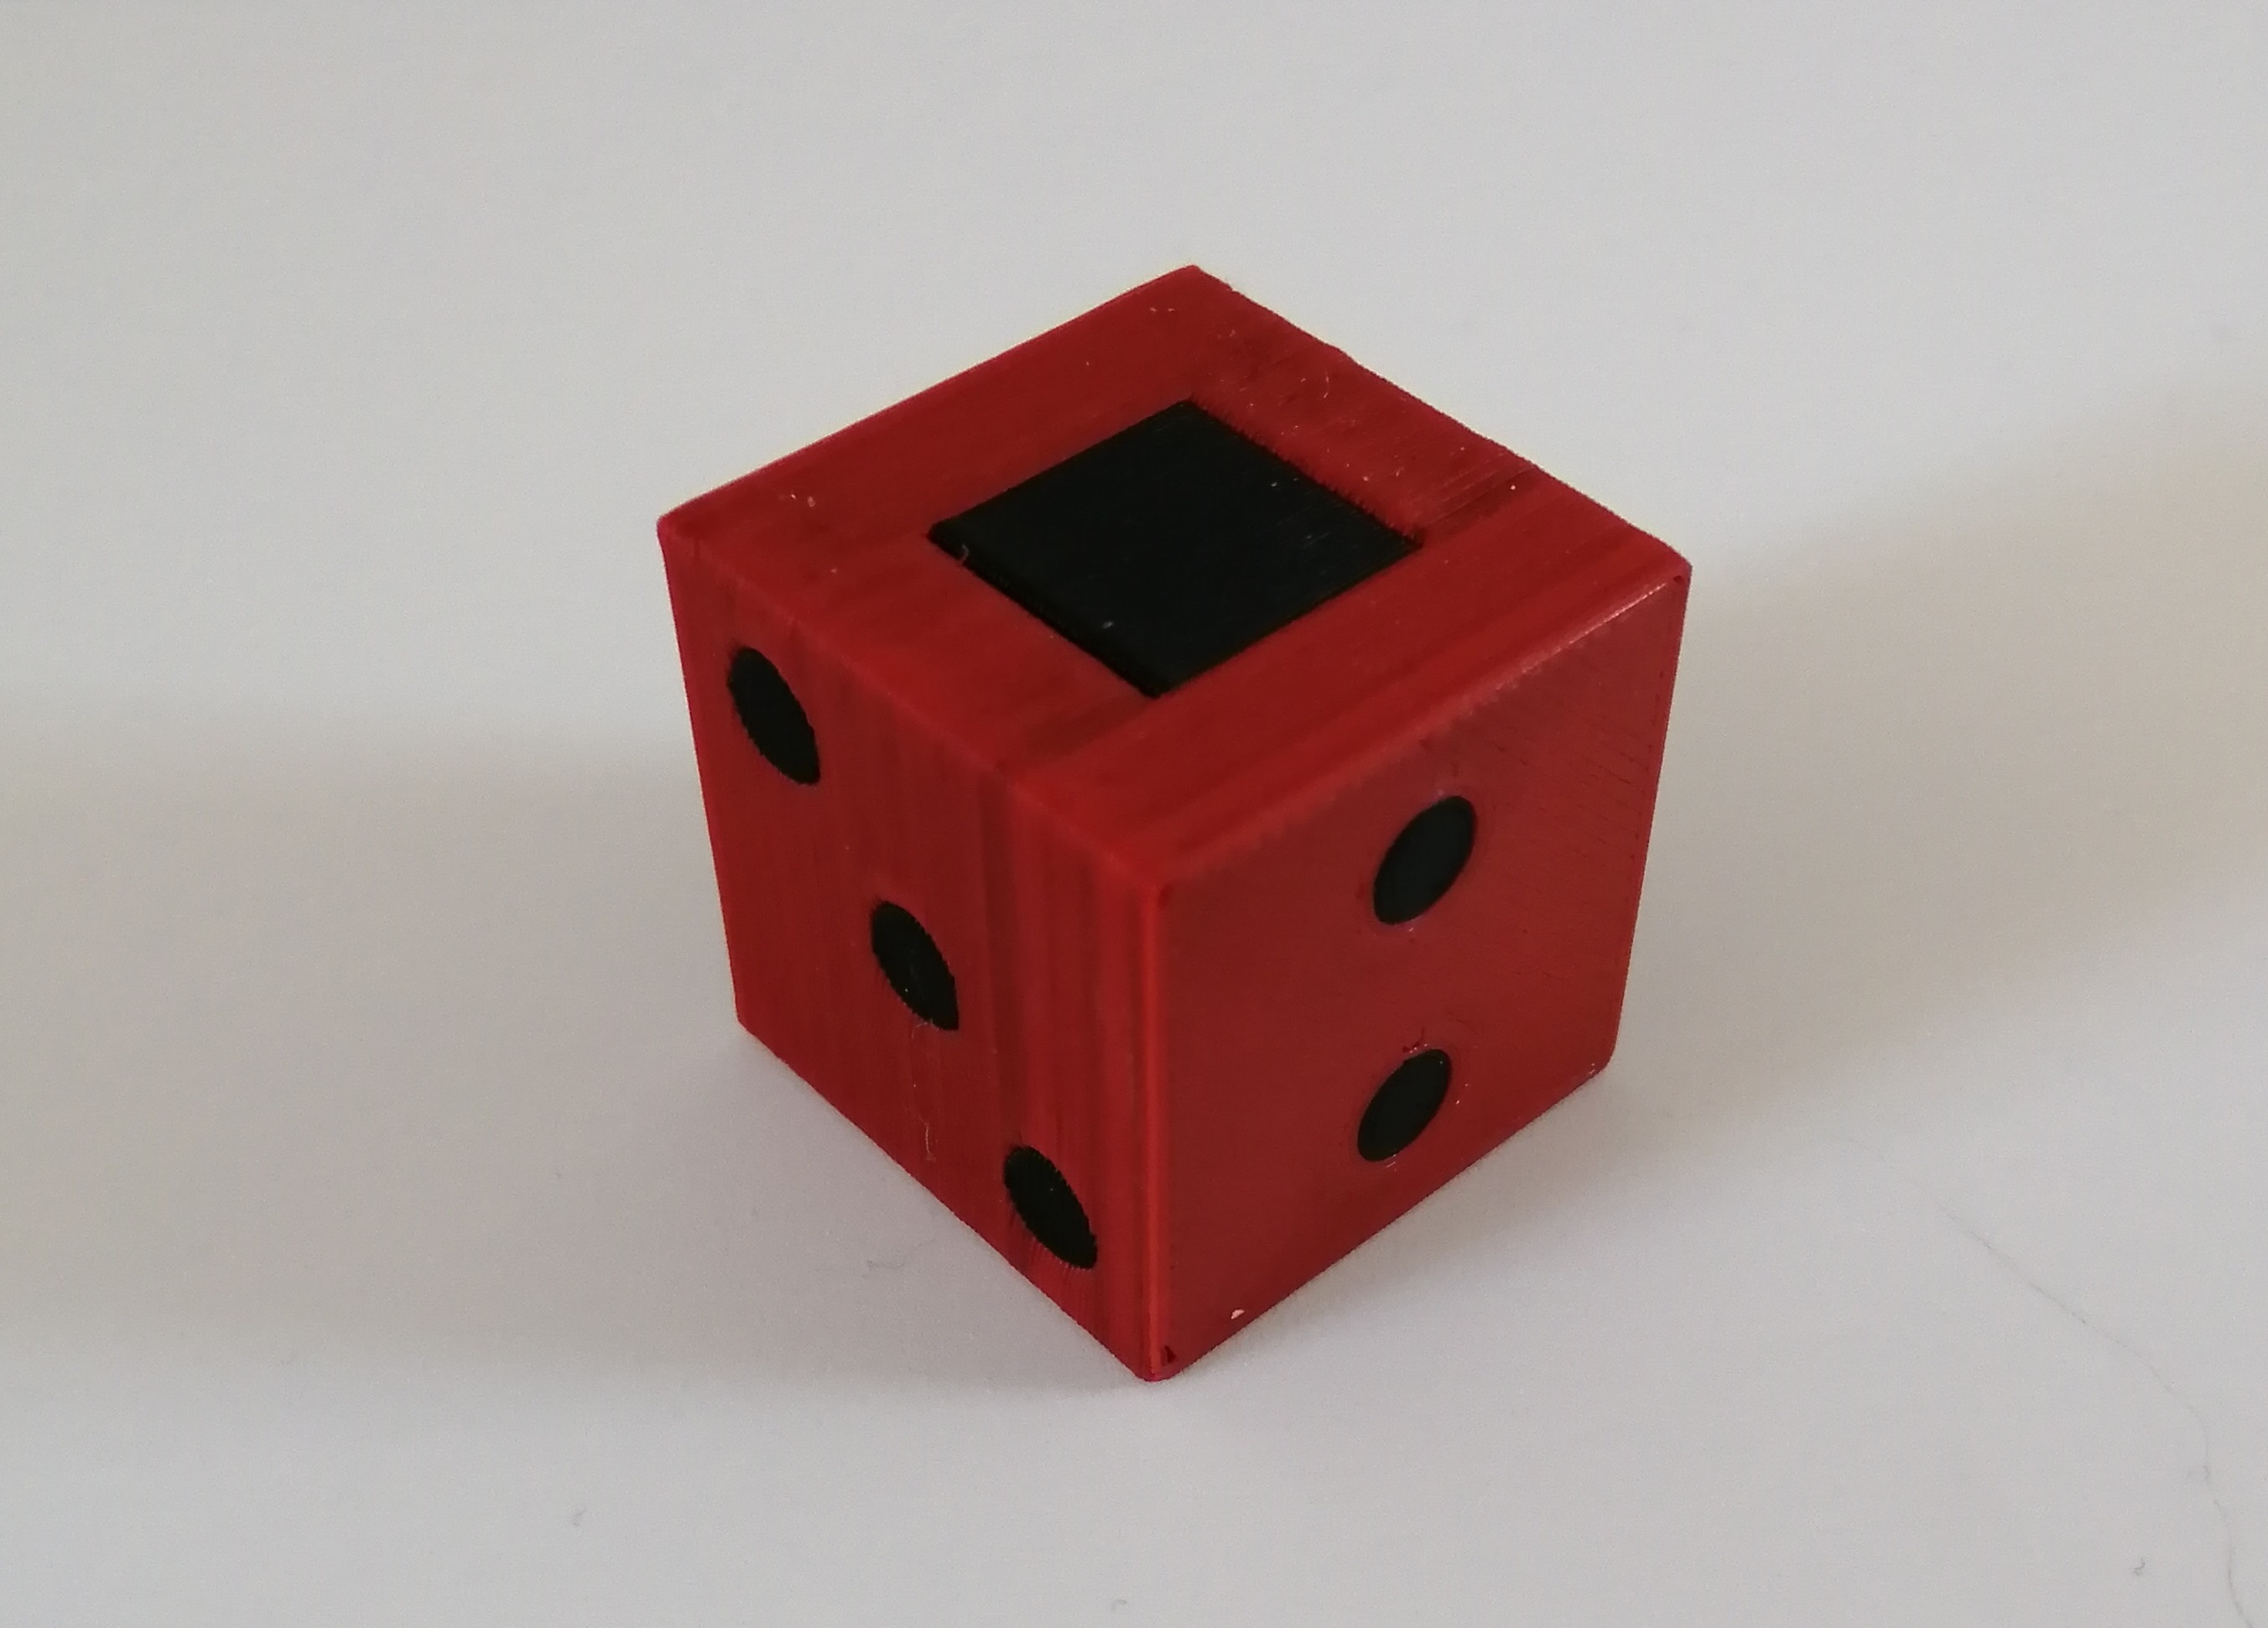
\includegraphics[width=.33\linewidth]{images/die_pic_general.jpg}
    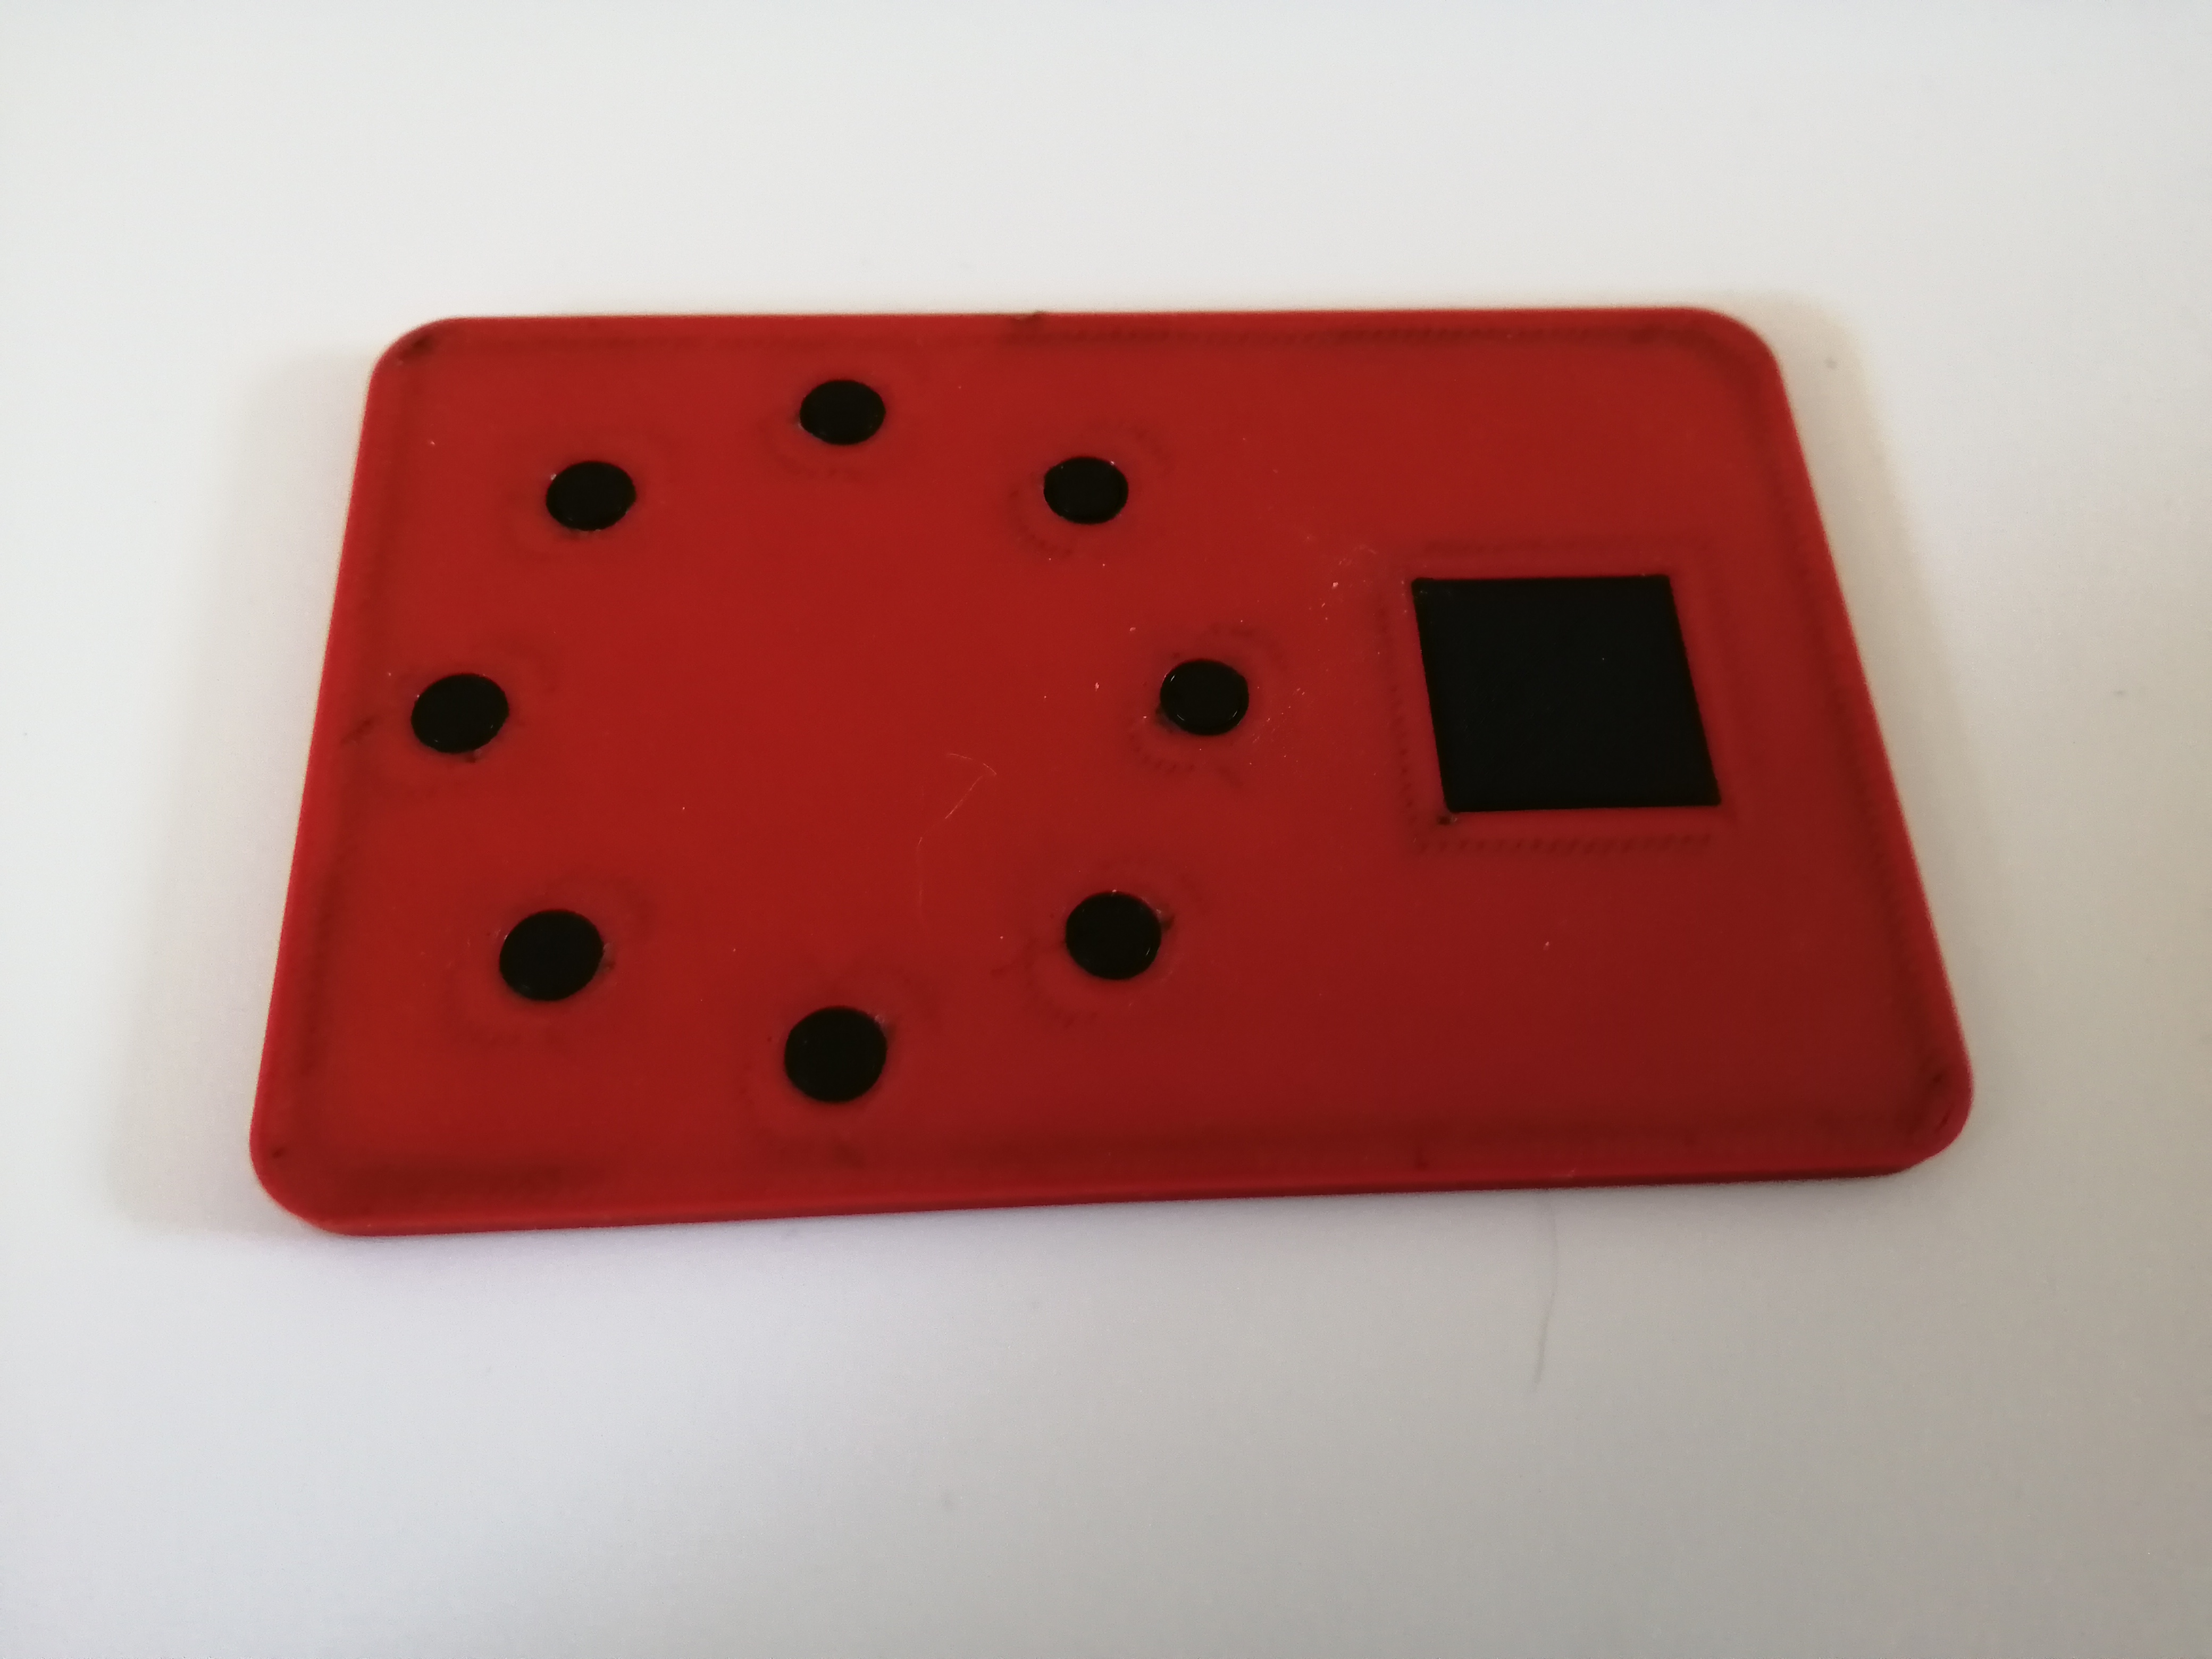
\includegraphics[width=.33\linewidth]{images/ccard_pic_general.jpg}
    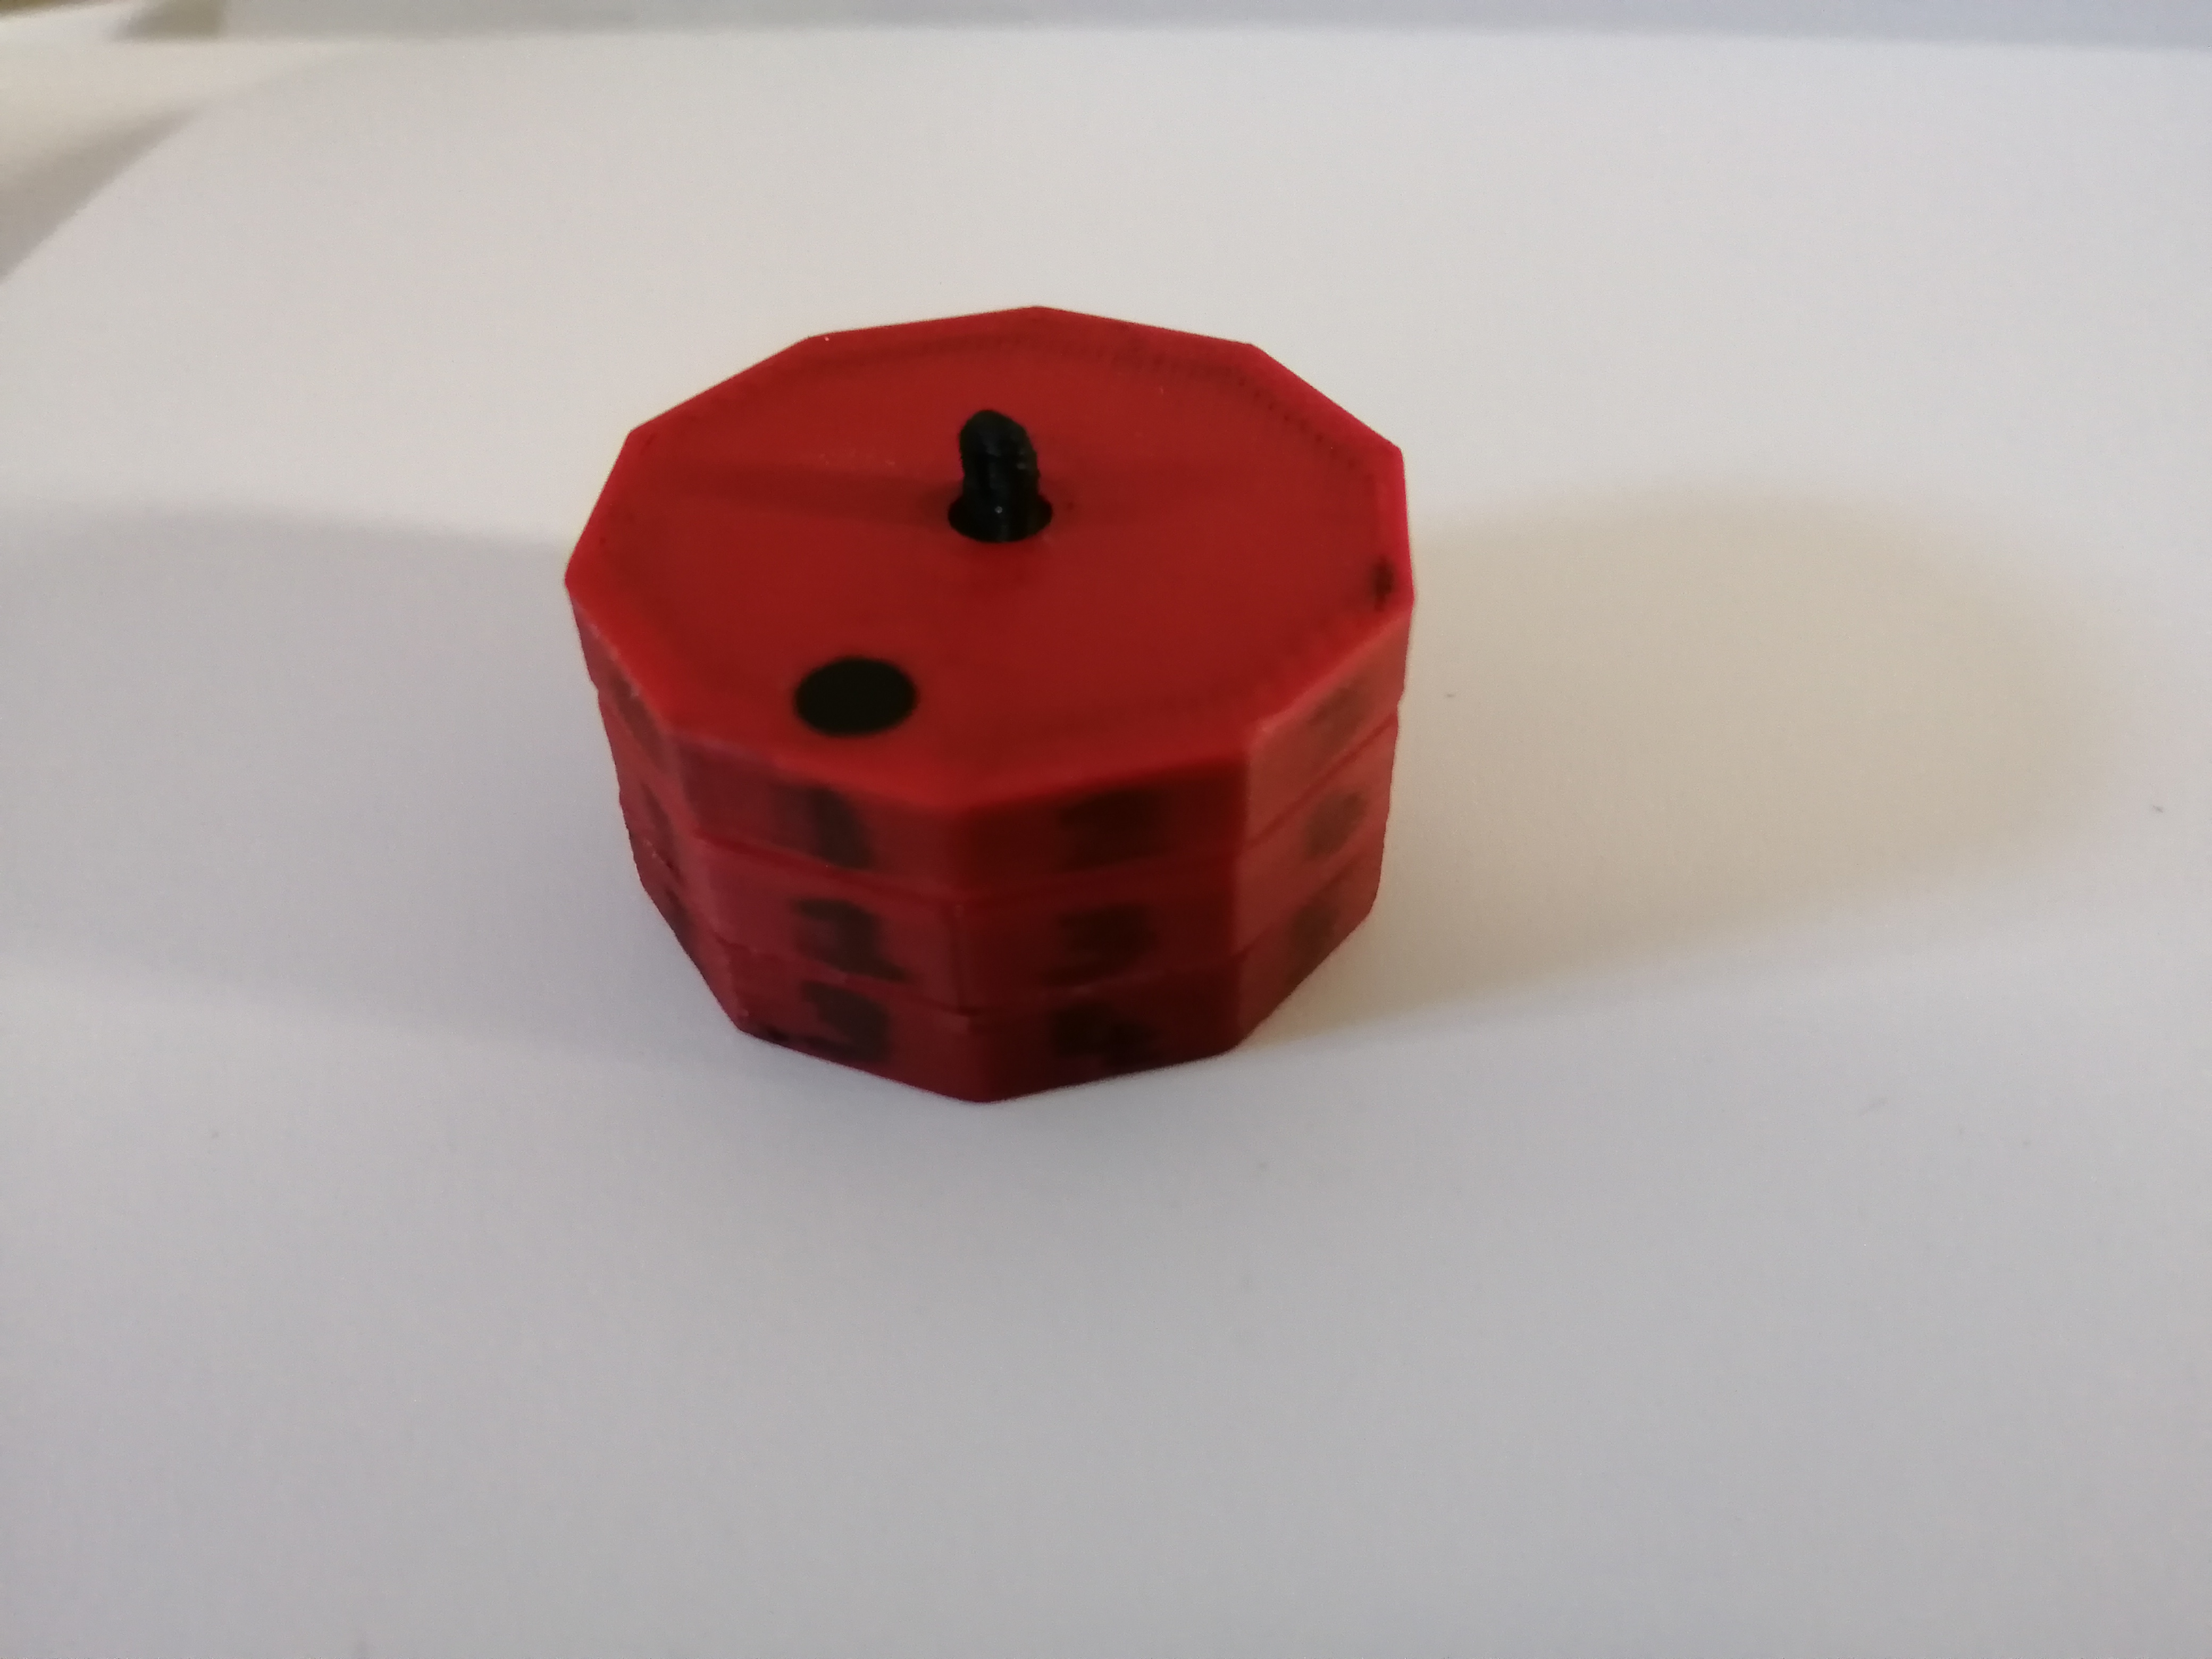
\includegraphics[width=.33\linewidth]{images/pendant_pic_1.jpg}
    \caption{The 3 models used in the study, the cube model (left), the card model (center) and the pendant model (right).}
    \label{fig:models}
\end{figure}


\subsection{Mock Authentication App} \label{ssecapp}
\label{sec:app}
A mock authentication app was required for this study to provide the participants somewhere to use their given object for authentication and mimic the need for authentication throughout the day by sending notifications. This also served to collect some data that would be useful in determining the usability of the authentication method.
 
The first task when creating the app was to define the list of initial requirements, as well as the platforms to build for. The app was decided to be created for Android in Java, as it was felt this would allow for the largest number of people to participate in the study, considered the simplest and most versatile to develop for, as well as already having access to the Google Play Store meaning it would be easy to install for participants. The requirements generated indicated there was a small amount of functionality that had to be implemented to be considered complete:
\begin{itemize}
    \item The app must be able to send notifications multiple times per day to remind users to authenticate, simulating the need for authentication throughout the day.
    \item The app must be able to register the authentication attempts made by the users.
    \item The app must be able to collect data on the authentication attempts and save to a log file for retrieval of the collected data at the end of the user study.
\end{itemize}
As well as this, it had to be decided what data to collect during the authentication attempts, the final list of data collected being \textit{participant number and model provided, when the authentication attempt took place, whether the authentication was a success, the number of attempts it took, how long it took}, as well as \textit{a user input indicating where they were when they authenticated.}

The app was created a built to meet each of the requirements one by one, with notifications being dealt with first: using a random number generator the interval until the next notification was set upon opening the app (resulting in only one notification at a time) then scheduled to be sent using Android's Alarm Manager package. In addition, notification were specified to only be sent during the hours of 8a.m. and 9p.m., ensuring that they are only received during the day, achieved by checking if the random notification delay generated fell between these hours and setting the delay to reflect this constraint. This was followed by logging of the required data which was extracted into a utility function class, both of which proved to be no issue. However, this gave rise to new requirements for the application: the app must provide a method to save the log file into accessible storage on the device (e.g. the /downloads folder); the app should provide a way to test the functionality of all implemented methods (e.g. notifications, saving the log file); the app should provide a way to change the authentication model without having to reinstall the app completely (to facilitate the 3rd stage of the exit interview).

Implementation of the app proved to be complex, as some of the methods required for use in authentication validation worked inconsistently across different devices and Android versions, returning blank or unhelpful data from essential functions, in particular the following functions: 
\begin{lstlisting}[language=java]
MotionEvent.getHistoricalPointerCoords() 
MotionEvent.getSize()
\end{lstlisting}
Since the app was to be deployed on potentially many different Android smartphones during the field study (as participants were to be asked to use their own mobile devices), it had to be built such that authentications could take place on any device running Android, meaning these methods could not be used. As a result, the authentications were limited to using the number of touchpoints on the screen at once, as well as the location of the touch points, the impact of which will be discussed in Subsection \ref{ssecmodels}. This was not the only method of validation investigated for use, with the use of raw capacitive data considered initially, as used in ItsyBits [\cite{schmitz2021itsy}], however this proved to also be an issue, as accessing raw capacitive data on Androids required root access, which was deemed to be too invasive to use during the field study.

The final implementation utilised views to capture touch actions and upon detecting a MotionEvent.ACTION\_UP, the data captured from ACTION\_DOWN events were sent to a function in the view's encapsulating activity which checked the registered model and dealt with authentication attempts.

Each object would be required to have its own validation method, hence it was decided that each model should take the form of a class inheriting methods from a parent abstract class outlining a general authentication model. This allowed for any number of the models designed to be implemented in the app providing good scalability. The models implemented are as outlined in Subsection \ref{ssecmodels}.

The app itself was built using Android Studio and tested manually using a physical Huawei PSmart 2019 running Android 9, as well as an emulated Google Pixel 2 running Android 10 and 11. A limited test bench was implemented, however it only tested the notification scheduling. All defined requirements were successfully met by the completed application and built into an APK, with a second release APK being built specifically for Android 10, due to the permissions required for writing to external memory being different from other versions, and a lack of time to completely implement the change into a single version.



%==================================================================================================================================
\chapter{Evaluation}

In this section, the methodology of the study in the wild is discussed along with the results of the evaluation.

\section{Methodology}

To assess the usability of the models designed and the authentication method as a whole, an exploratory study was performed as outlined with three participants.

\subsection{User Field Study}

The purpose of performing the study was to assess how users interacted with the tangible authentication method in their daily lives over an extended period, hence a lab study would not have been sufficient. The study took place over one full week, consisting of an initial meeting, multiple daily mock authentications, and finally an exit meeting.

In the initial phase, participants were required to be present for an in-person meeting. The procedure of this meeting was as follows, and adheres to the BPS ethical guidelines:
\begin{itemize}
    \item  \textbf{1 - Familiarizing participants with the project.} Upon arrival, participants are greeted and informed about the concept of tangible two-factor authentication, as well as what they would be required to do over the week. To do so, an introduction script was designed to be read with the opportunity for any questions clearly indicated before agreeing to participate. Here it is also made clear what data will be collected and that it will be stored in accordance with the GDPR.
    \item \textbf{2 - Gathering informed consent.} Having explained the purpose behind the project, as well as what would be required of them, the participants were each asked to sign a consent form indicating they have understood what has been explained and that they agree to take part.
    \item \textbf{3 - Demographics survey.} Each participant is assigned a participant number and asked to fill out a demographics survey, consisting of basic demographic questions as well as a set of questions to find their affinity for technology (the contents of this survey can be found in Appendix Section \ref{sec:demo}).
    \item \textbf{4 - Introduction to the object.} The participants were then assigned one of the three final models to use for the next week, as well as the mock authentication app installed on their mobile device. An information sheet demonstrating how to interact with the object is provided as well as a demonstration by the interviewer, and time is allotted to allow for the participants to get familiar with the object and method of interaction. Here all the methods in the app will also be checked for functionality on the device.
    \item \textbf{5 - Schedule final meeting.} Having received all of the necessary information and with the setup complete, the participants are asked to schedule a second meeting for the end of the study at least one week from the day, and any additional questions they have are answered before the end.
\end{itemize}

Upon completion of this initial phase, participants were to go about their daily lives as normal, ensuring that their designated model is with them, and checking for notifications from the app. Upon receiving a notification (or upon noticing a notification) from the app, participants were to perform an authentication, with three attempts to succeed. This would involve launching the study app, pressing the button to begin an authentication attempt, and interacting with their designated model as demonstrated in the initial meeting, then finally inputting where the authentication took place. Each of these authentications was considered to take a maximum of five minutes, and the participant was asked to perform at least two per day. 

Once the week had concluded, the participant was asked to be present for another meeting previously scheduled. The procedure of this meeting was as follows:
\begin{itemize}
    \item \textbf{1 - Re-familiarising.} The participant was greeted and reminded of the purpose of the study.
    \item \textbf{2 - Exit survey.} They were then asked to fill out an exit survey to gather the system usability score for the application method, as well as gather some extra information regarding the continued function of the object. During this time, data collected by the app is to be extracted from the mobile device.
    \item \textbf{3 - Exit interview.} Upon completion of the survey, the participants are asked to take part in a recorded interview and assured once again that the data they provide will be anonymous and recordings will be transcribed and deleted. The interview has 3 stages:
    \begin{itemize}
        \item Stage 1 - Participants are asked questions about their week using the item
        \item Stage 2 - Participants are asked about their perception of two-factor authentication in a general sense and concerning the project specifically
        \item Stage 3 - A short break is taken allowing for participants to experience using the other two models, then asked their opinions on them, as well as on 3D printing in general.
    \end{itemize}
    The complete script can be found in Appendix Section \ref{sec:interview}. Upon completion, participants are offered a chance to ask any other questions or give their comments before leaving, as well as provided contact information for the investigator if they have any comments or questions after leaving.
\end{itemize}


\subsection{Demographics}

Recruitment for the participants was done through mailing lists as well as word-of-mouth. Each of the participants was required to be over 18 years of age, as well as own an Android phone. The final demographics information for the participants can be found in Table \ref{tab:demographics}. Each of the participants was compensated with a £40 Amazon voucher for their time at the end of the study.

\begin{table}[]


\resizebox{\textwidth}{!}{\begin{tabular}{l|lllllll}
\toprule
ID & Age      & Gender & Country of Residence & Job      & Work from Home & Two Factor & ATI  \\
\midrule
P1              & 26-30    & Male   & Scotland             & Employed & Yes            & Yes        & 4    \\
P2              & 21-25    & Male   & Scotland             & Student  & Yes            & Yes        & 4.44 \\
P3              & Under 21 & Female & Scotland             & Student  & Yes            & Yes        & 3.44 \\
\bottomrule
\end{tabular}}
\caption{Demographics information for the participants collected in the initial meeting during the study.}
\label{tab:demographics}
\end{table}
\newpage
\section{Results}

Here results will be presented in two parts: \textit{Qualitative data} and \textit{quantitative data.}

\subsection{Quantitative}
Here the data collected by the application during the study is outlined, in addition to the results from the exit survey.

One of the metrics gathered by the study application measures the time taken to complete an authentication attempt. Since the overall time for the authentication was collected, this time was divided by the number of attempts taken to find an average time for each attempt across one authentication. The overall average time taken for each of the models is indicated in Table \ref{tab:quant} as well as the standard deviation. The object with the overall fastest average time per attempt was the card model with 5.16 seconds per authentication (max = 15.51, min = 2.65, SD = 2.68). This is followed by the pendant model with 5.47 seconds per authentication (max = 12.29, min = 2.29, SD = 3.49). And lastly, the overall slowest average time per attempt was found in the cube model with 8.09 seconds per authentication attempt (max = 19.06, min = 2.03, SD = 3.67). The development of time taken per attempt can be seen for each of these models in Figure \ref{fig:time_taken}.

In addition to the collection of authentication time, the success rate was also measured by taking the number of successful attempts over the total number of attempts, with the highest overall success rate found with the card object (53.66\%), followed by the pendant (23.4\%) and the cube (15\%). As well as on an attempt basis, the success rate was also measured on an authentication basis - that is, how many full authentication attempts resulted in a success, which showed again the card object had the highest success rate (88\%), followed by the pendant (61.11\%) and the cube (38.71\%). These numbers can also be found in Table \ref{tab:quant}.

Finally, during the exit meeting, the users were asked to complete a survey with a section for the system usability scale. The final scores indicate the perceived usability of both the object and authentication app together, with an overall average of 57.5.

\begin{table}[]
    \centering
    \resizebox{\textwidth}{!}{
    \begin{tabular}{cc|c|cc|cc}
         \toprule
         ID & Object & SUS & Mean Time (s) & SD & Success Rate (Attempt) & Success Rate (Authentication) \\
         \midrule
         P1 & Cube & 60 & 8.09 & 3.67 & 15.00 & 38.71\\
         P2 & Card & 52.5 & 5.16 & 2.68 & 53.66 & 88.00\\
         P3 & Pendant & 60 & 5.47 & 3.49 & 23.40 & 61.11\\
         \bottomrule
    \end{tabular}}
    \caption{Table detailing the quantitative results for each participant and model}
    \label{tab:quant}
\end{table}

\begin{figure}
    \centering
    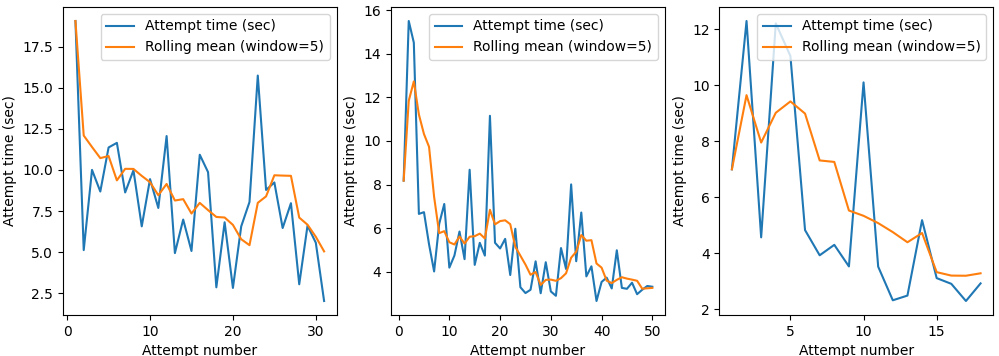
\includegraphics[width=\linewidth]{images/timetaken_with_rolling_mean.png}
    \caption{This figure illustrates the improvement in authentication time over number of attempt for each of the 3 participants.}
    \label{fig:time_taken}
\end{figure}

\subsection{Qualitative}

Here the findings from the exit interview will be outlined, with transcripts of the meeting being analysed via thematic analysis as outlined by \cite{braun2012thematic}. This resulted in 5 main categories: \textit{Security, How it feels to use, Method of use, 3D printing and Commercial} in addition to any recommended improvements.

\textbf{Security}\\
All of the participants in the study were familiar with the use of two-factor authentication, each citing different established methods that they had to use often, however two of the participants only used the methods when they were required to, with one (P2) saying the reason they do not often activate it is because they feel like they have nothing worth stealing.

When asked about how secure the model feels to use, two of the participants were unsure (P1, P2), with one noting that they felt vulnerable to shoulder surfing attacks. Interestingly, P2 mentioned that \textit{"[they] realise how secure it is, and it is quite secure, but it doesn't necessarily feel like it."} and felt that it \textit{"feels a bit like a toy"}.

Speaking about the physical security of the objects, two of the participants explicitly spoke about how it was unlikely for the objects to be stolen:
\begin{itemize}
    \item \textit{"I didn't leave the item out on a tabletop... I always carried it with me so not that much danger of it being stolen"} (P1)
    \item \textit{"It would be really inconspicuous. No-one would have any idea what it is"} (P2, on the cube object)
\end{itemize}

\textbf{Usability}\\
This was the largest category that was found, linking the closest to the issue of usability during the interviews.

On the initial use of the model, two of the participants discovered a bit of a learning curve (P1, P2), with P1 mentioning they often touched the screen with their fingers during attempts at the beginning of the study. The same participants also mentioned that they felt at least one of the models was fragile, with P1 mentioning the pendant model felt fragile \textit{"On account of it having moving parts"}, however P2 later began to feel more confident in the strength of the card model - \textit{"I did worry about it actually breaking, but never managed to break it. You wouldn't be able to"}.

While all of the participants agreed that the model was easy to carry with them, they all disliked using them with phone in hand rather than on a tabletop or other flat surface, generally avoiding doing so. Each of them also mentioned that the models tended to slide on the phone screen, which led to failed authentications.

It was also brought up by two participants that it was felt that there was not enough feedback when authenticating, and it was difficult to tell if something went wrong, or what caused a failure. Each of the participants also felt that authenticating was inconsistent in its current state with one participant summing it up: \textit{"Some of the time the authentication just wouldn't go through"} (P3).

Throughout it interview each of the participants also spoke about the enjoyment factor, expressing that the method was fun to use, adding to the usability, while two of the participants mentioned that the familiarity of the model and the method of interaction was also important.

Finally, each of the objects was well-liked and discussed in such as way by at least two of the participant, with the card model drawing two participants to call it their favourite, while the last preferred the cube object the most. It was also mentioned by each participant that they would prefer to use this method over other two-factor methods, with P2 adding \textit{"at least in some scenarios"}.
\newpage
\textbf{Method of use}\\
Participants were also asked about where they would prefer most to use it, and while all agree they would mainly use it for services where two-factor authentication was already implemented (systems like banking apps), there was more of a range when discussing the devices and locations. P2 stated \textit{"I'm not sure if smart phones [are] the best place to use it"} and said they would prefer to only use it at home, so stationary devices would be best, but the other participants were willing to use the method on any device that allowed it. In terms of location however, P3 agreed is was \textit{"definitely easier to use it at home than when I'm out."} and would prefer to use it on services they don't open a lot.

\textbf{3D printing}\\
To get a sense of how the objects could be distributed, the participants were also questioned about their opinions of 3D printing. While there was a range of answers on whether or not the participants would buy them, they all mentioned that they thought there would either be widespread adoption or in-person services available (like existing \textit{"copy-shops"} (P1)) that would allow for printing to be done without owning a 3D printer.

\textbf{Commercial}\\
Finally, when asked if they would purchase the models for use, two of the three participants were hesitant to:
\begin{itemize}
    \item \textit{"I don't know... I feel it would be more used for banks"} (P3)
    \item \textit{"I would consider but I don't think I would end up buying... It's more cumbersome than not at all"} (P1)
\end{itemize}

%==================================================================================================================================
\chapter{Discussion} 

In this paper, the usability of tangible two-factor authentication using conductive and insulating PLA and capacitive touch screens has been investigated. In this section, the results of the study will be discussed, along with the limitations of this paper, as well as potential future directions that may be promising for research.

\section{Results and Improvements}

%result discussion
The preliminary results of this study proved promising - while the objects performed inconsistently in the field due to failings in the implementation, the time taken to use them per attempt was shown to improve as the participants grew more experienced using them, with minimum times found towards the end of the study period on the order of only two seconds. This sentiment was also expressed by the users themselves, with two participants noting the learning curve during the interview section. When compared with other contemporary methods of two-factor authentication as investigated by \cite{reese2019usability}, we can see that in terms of timing, this method is comparable to the use of codes (mean 2.2 seconds), and far faster than more complex methods like U2F security keys (mean 57.8 seconds). Hence, it should be noted that to properly assess usability with new designs of tangible two-factor authentication objects following this paradigm, time must be allowed for users to become familiar. 

%result discussion
Although, while this metric proved to be favourable, the success rate of authentications proved worrying, with very low rates of success per attempt. However, this was not due to a problem with the objects, or the method of interaction, as each of the participants noted that at least one of the models did not consistently authenticate in the application, despite actions being performed correctly. This was due to the capacitive resolution of the touch screen - since the models were designed with usability in mind, and respondents in the initial survey desired smaller, more portable objects, it follows that any conductive points interfacing with the touch screen would be close together because of the limited space on the object, resulting in an inconsistent read as multiple touch points are registered as one. In addition, this was affected by the implementation of the authentication app, with the issues previously discussed in Section \ref{sec:app} resulting in a flawed design. As a result, it can be seen that the perceived usability of the method was reduced, with a mean SUS score reflecting this, far lower than each of the methods explored by \cite{reese2019usability}.

%result discussion
Another interesting result indicated that for the more technically adept users who participated, the security of the authentication method felt more flimsy, with one participant noting the difference in expectation between their perception of security and the reality of using the item - they were aware that on paper it is secure, but due to the simplicity of using it, felt that it couldn't be secure. This brings to light a perception some users may have of two-factor security - that it must be complicated and difficult to use for it to be truly secure. This same user noted that the pendant model - the model that adapted a combination lock style of interaction - felt the most secure of the objects, despite having the solution to its interaction easily accessible by taking it apart - a potential security issue that future research in this area should consider for objects such as this one, whether by adding an extra interaction or via adding 'decoys'. This seems to indicate that for some users, interactions should feel comparable to existing security measures for tangible authentication methods, indicating that perhaps rather than novel and enjoyable interactions, some users would prefer familiar actions that they already link with security for assurances that the method is truly secure. This disparity between user perception and reality has been noted before, such as by \cite{zimmermann2020password} who noted that not only can this be found in the security of a method, but also in the usability, with perceptions affected by multiple factors.

%result discussion
A usability issue brought up by participants was the material of the object, while strong its interaction with the phone screen resulted in difficulties for touch-based objects as the model easily slid out of place. It was suggested that a clip or some kind of holder be given alongside the object to make authentication easier, however this would create more overhead, a problem which resulted in assembly interactions being ejected from the study. While utilising a different material for the non-conductive parts of the object would increase issues with distribution, this appears to be the simplest solution to this problem and should be considered in future work.

%result discussion
Another trend found during the study indicated that many potential users of this authentication method preferred to keep the models for use at home with services they use rarely. As such, perhaps the focus this study had on making small and portable models was misguided, and a case could be made rather for focusing on larger, more complex models to be used solely in the home. This may also prove advantageous in the retention of users, as emphasis on portability will require users to build habits around the method, whether bringing the object with them when going outside or simply keeping it nearby, which may put some users off. At least in this current stage, it was clear the participants were not interested in using the objects more than they had to.

%improvement
An improvement often mentioned by the participants involved more feedback when performing the authentication. Allowing users to see the progress they've made during the process of authentication or some form of demonstration by the app that an interaction has indeed been registered, whether via haptic feedback, or audio cues, would greatly have improved user experience during the performed study.

\section{Limitations and Future Work}
%limitation
In finding the usability of the developed models, a clear limitation is the small sample size of participants drawn for the field study. As a result, the findings presented should only be considered a preliminary indication, and a follow-up study should be performed to investigate further and solidify understanding of the user experience of this concept.

%limitation and future
One of the large issues this project faced already touched upon was the inconsistency of the model due it the study applications implementation. Over the course of development, the inconsistency of Android touch event methods was a problem, as for the implementation to be considered a success, it should run on most phones. This limited how objects could be validated, leaving the actual implementation less than secure, with only position and number of simultaneous touch points able to be used, both of which are easily replicated without the object. To truly implement this kind of authentication, this paper recommends future works instead use raw capacitive data, making use of research already done in this area such as by \cite{schmitz2021itsy} who used machine learning for recognition of smaller object footprints and \cite{mayer2021super} who created a method of improving the low resolution of capacitive touch screens to better detect correct interactions. Future research could consider different methods of implementing the ownership factor - rather than the positioning of two or more dots, a QR-code-like implementation could be used as \cite{yu2011tuic} presents.

%==================================================================================================================================
\chapter{Conclusion}    

This paper investigated the usability of a method of tangible two-factor authentication through the design and creation of models and a mock authentication app, and assessed through data from a one-week-long user field study. Preliminary user feedback indicated that despite the usability issues, willingness to adopt this method as a form of two-factor authentication was high, and while not all participants were interested in a commercially distributed form, each expressed they would welcome tangible two-factor authentication once it had matured and offered improvements they would like to see. Ultimately, the outlook on this new method of authentication provided by the preliminary field study performed suggested that this is an area in which more research should be done, and that should the problems found by this paper be solved, it could well become a widely adopted tool in the future.


%==================================================================================================================================
\chapter{Acknowledgements}
This paper would not have been possible without the help of my colleague Laszlo Besenyei at the University of Strathclyde, who provided a great service in helping with the digital modelling of the objects, as well as Mohammed Khamis, who allowed me to intrude on his office for more than three months. I would also like to thank Karola Marky, my supervisor on this project, for lending her knowledge. 

Finally, I would not have been able to complete this without the support of my wonderful fianc\'ee, Elizabeth.

%==================================================================================================================================
%
% 
%==================================================================================================================================
%  APPENDICES  

\begin{appendices}

\chapter{Ethics Forms}

The appendices provide the relevant ethical information as used during the evaluation. A copy of the introduction and consent sheet can be found in Figure \ref{fig:intro1} and \ref{fig:intro2}, and the signed ethics checklist can be found in Figure \ref{fig:ethics1} and \ref{fig:ethics2}.


\begin{figure}
    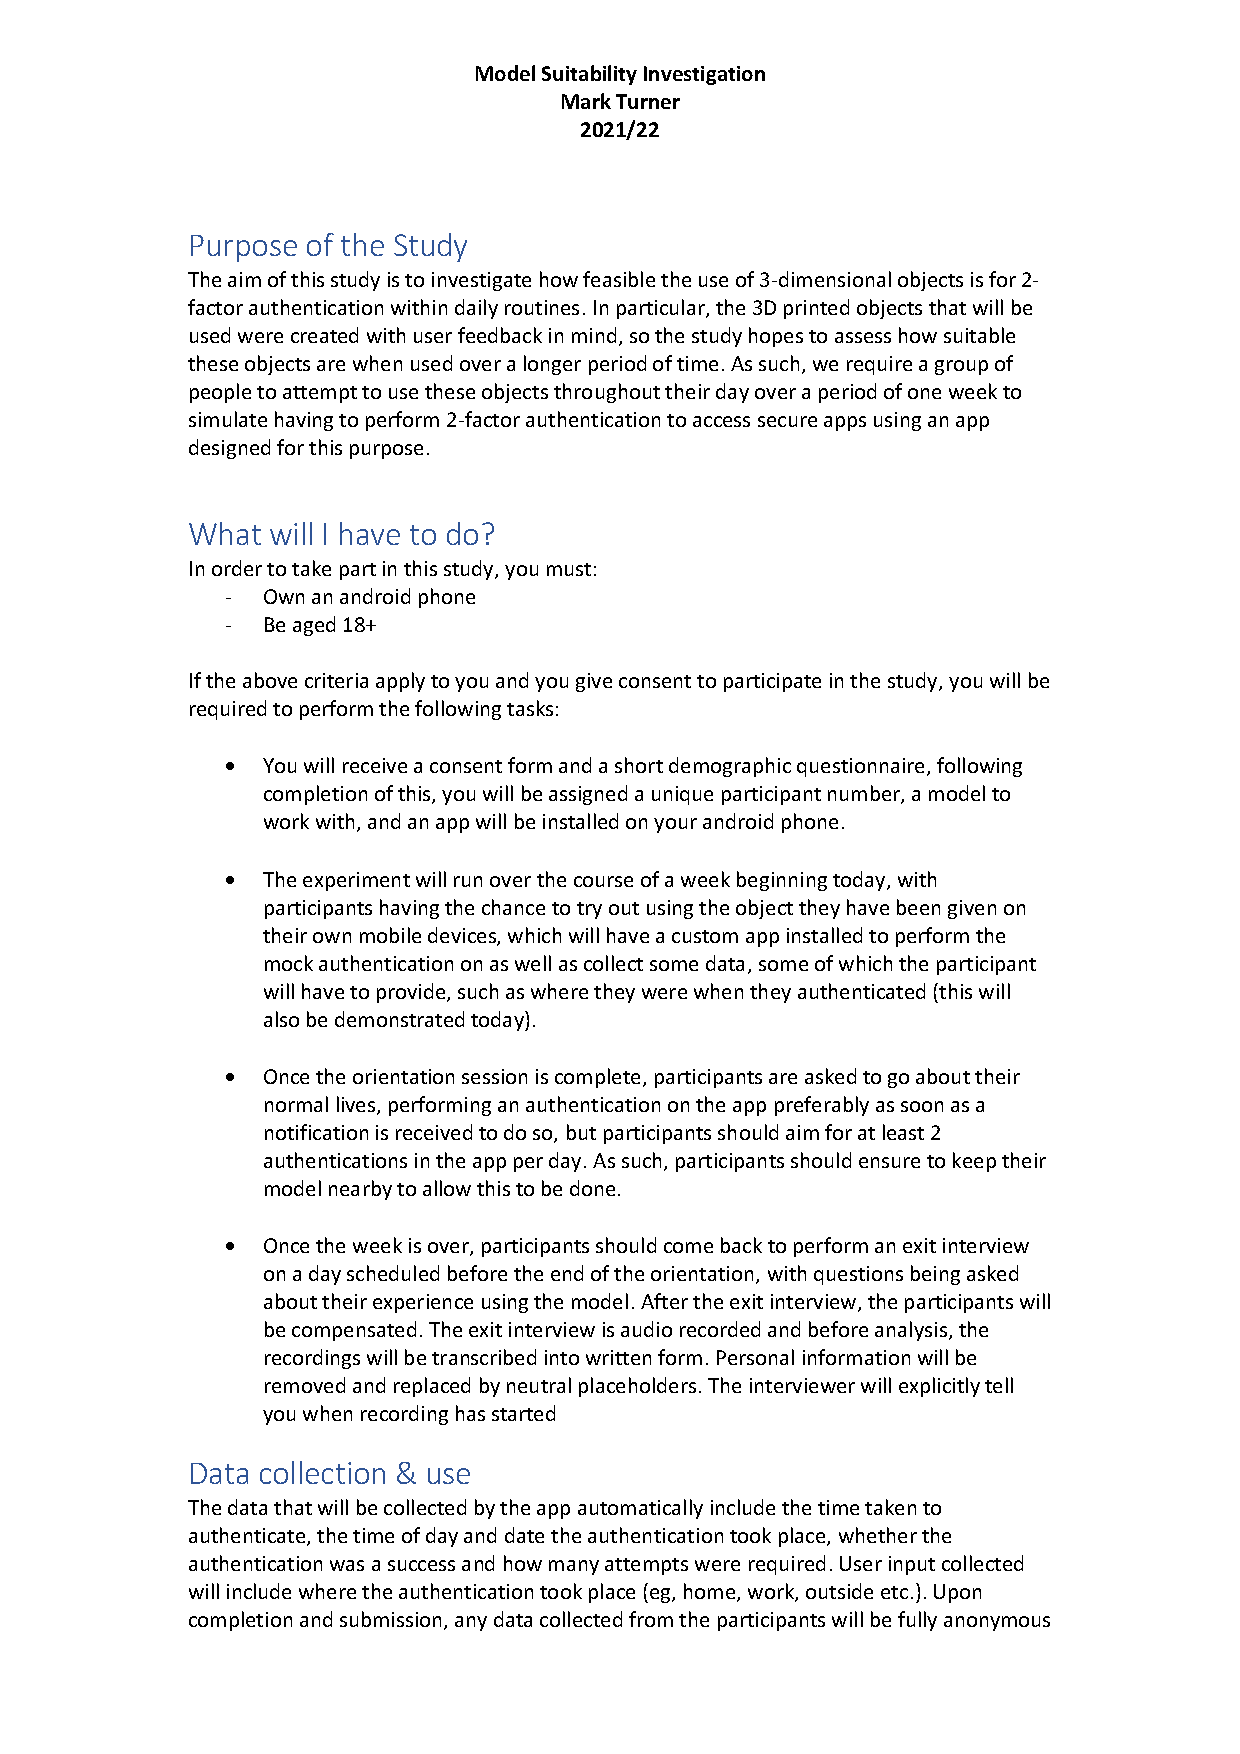
\includegraphics[page=1,width=\linewidth]{Appendices/introduction_script_and_consent_form.pdf}
    \caption{The introduction and consent form issued during the user study. (part 1/2)}
    \label{fig:intro1}
\end{figure}

\begin{figure}
    \includegraphics[page=2,width=\linewidth]{Appendices/introduction_script_and_consent_form.pdf}
    \caption{The introduction and consent form issued during the user study. (part 2/2)}
    \label{fig:intro2}
\end{figure}

\begin{figure}
    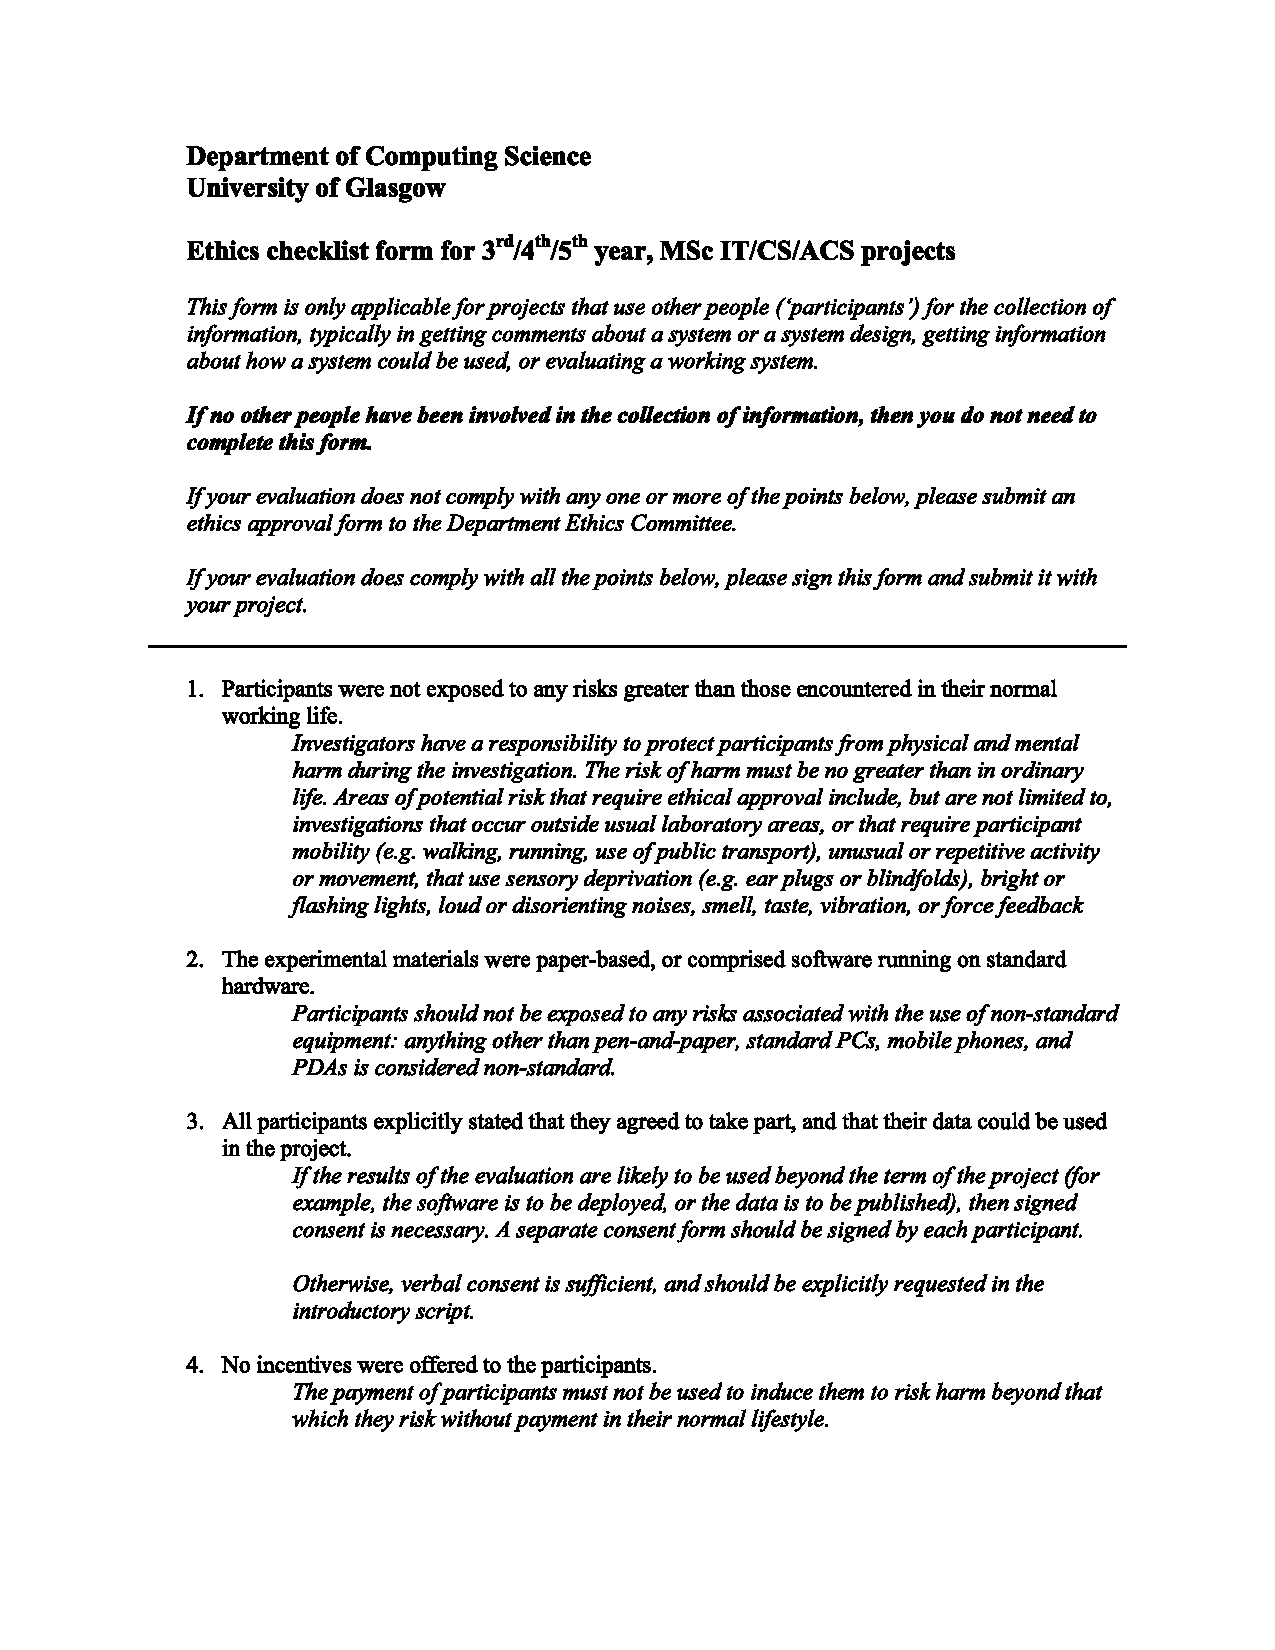
\includegraphics[page=1,width=\linewidth]{Appendices/ethics_form_KM.pdf}
    \caption{Signed ethics checklist. (part1/2)}
    \label{fig:ethics1}
\end{figure}

\begin{figure}
    \includegraphics[page=2,width=\linewidth]{Appendices/ethics_form_KM.pdf}
    \caption{Signed ethics checklist. (part2/2)}
    \label{fig:ethics2}
\end{figure}

\newpage

\chapter{Online Survey Analysis}
\label{sec:onlineana}

The following tables outline the findings of the analysis of the online survey performed prior to this study. After filtering for understanding, the number of valid responses numbered 88. The table of responses for size can be found in Table \ref{tab:modsize}, and for shape in Table \ref{tab:modshape}.

\begin{table}[H]
    \centering
    \begin{tabular}{c|c}
         Size (cm) & Number of responses \\
         \midrule
         1 & 4 \\
         2 & 8 \\
         3 & 19 \\
         4 & 4 \\
         5 & 34 \\
         6 & 7 \\
         7 & 3 \\
         8 & 4 \\
         10 & 26 \\
         12 & 2 \\
         13 & 1 \\
         15 & 8 \\
         20 & 2 \\
         30 & 3 \\
         45 & 1 \\
         50 & 1
    \end{tabular}
    \caption{The number of responses for a particular size of model suggested}
    \label{tab:modsize}
\end{table}

\begin{table}[H]
    \centering
    \begin{tabular}{c|c}
         Object shape & Number of responses  \\
         \midrule
         Cube & 17 \\
         Circle/coin & 13 \\
         Credit card/Rectangle & 11 \\
         Square & 7 \\
         Wearable (ring) & 5 \\
         Animal & 4 \\
         Necklace & 2 \\
         Keyring & 2 \\
         Phone case & 2 \\
         Car key & 1 \\
         Polygon & 1 \\
         Cylinder & 1 \\
         Fidget Spinner & 1 \\
         Car & 1
    \end{tabular}
    \caption{The suggested shape of the models and the number of occurrences}
    \label{tab:modshape}
\end{table}

\clearpage

\chapter{Production Sketches}
\label{sec:prod}

The production sketches created during development of the objects can be found in Figures \ref{fig:prod1}, \ref{fig:prod2} and \ref{fig:prod3}

\begin{figure}
    \centering
    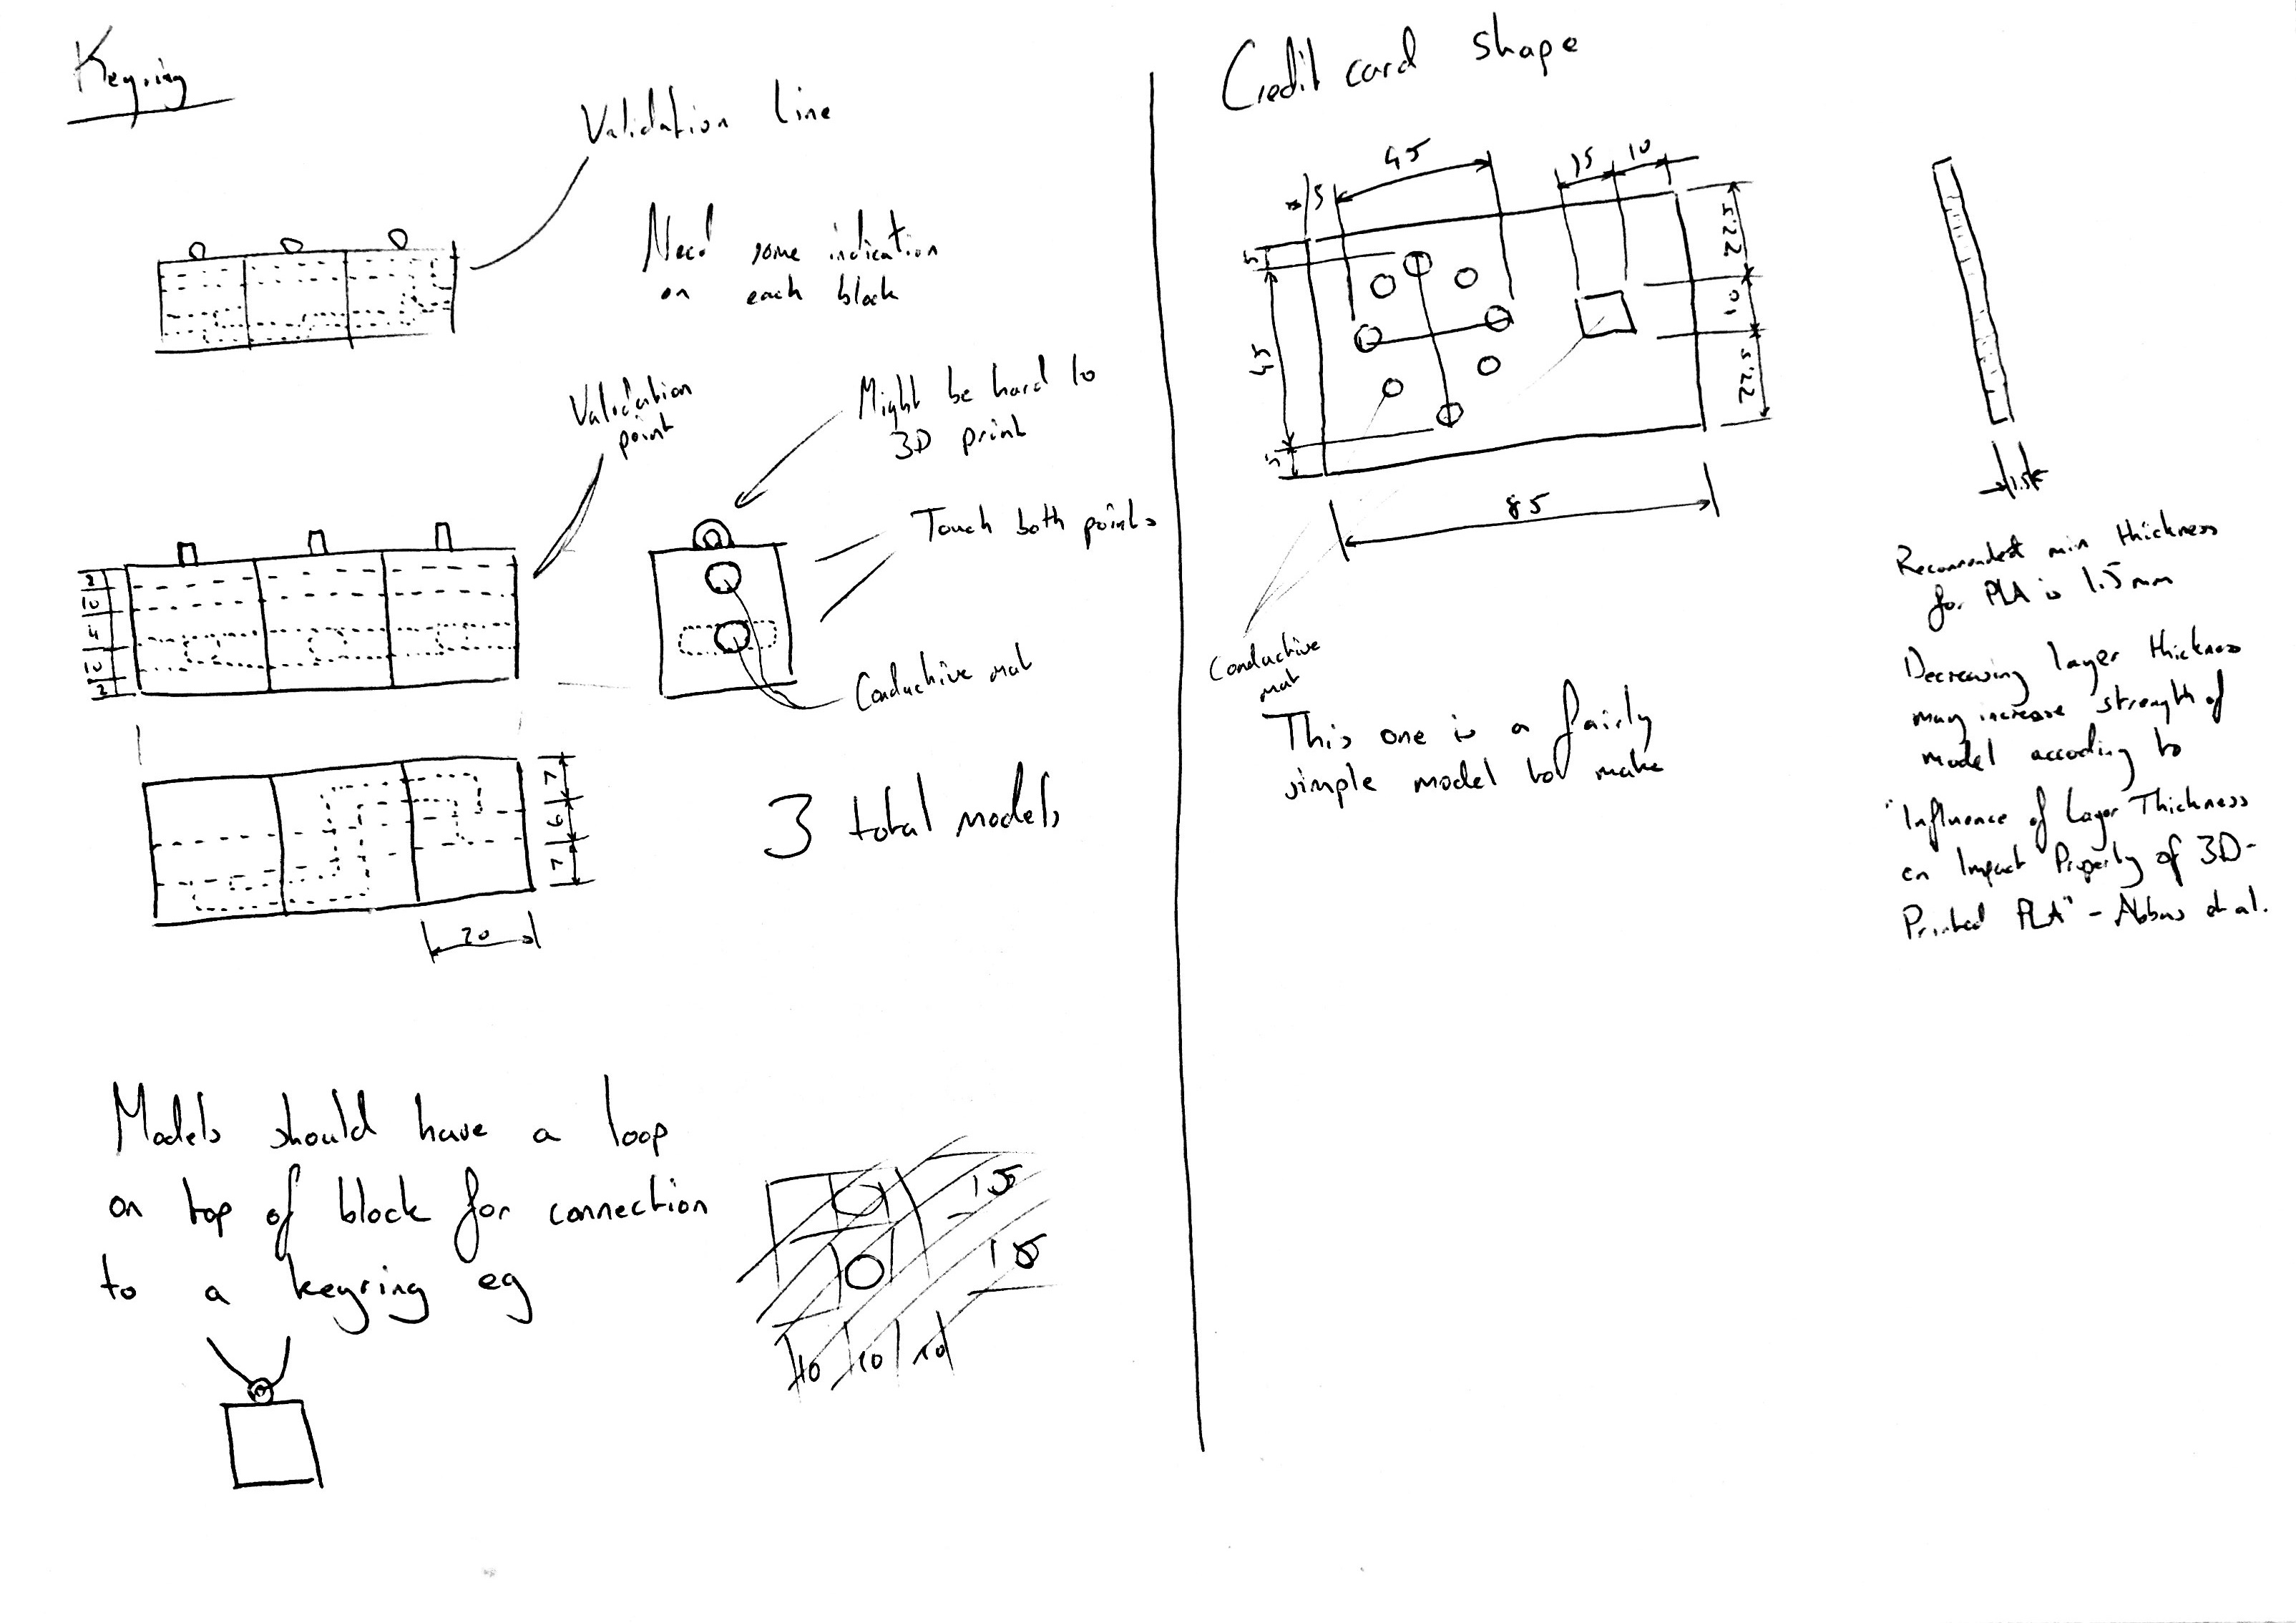
\includegraphics[width=\linewidth]{Appendices/prod_1.jpg}
    \caption{Initial production drawings for keyring and credit card models}
    \label{fig:prod1}
\end{figure}

\begin{figure}
    \centering
    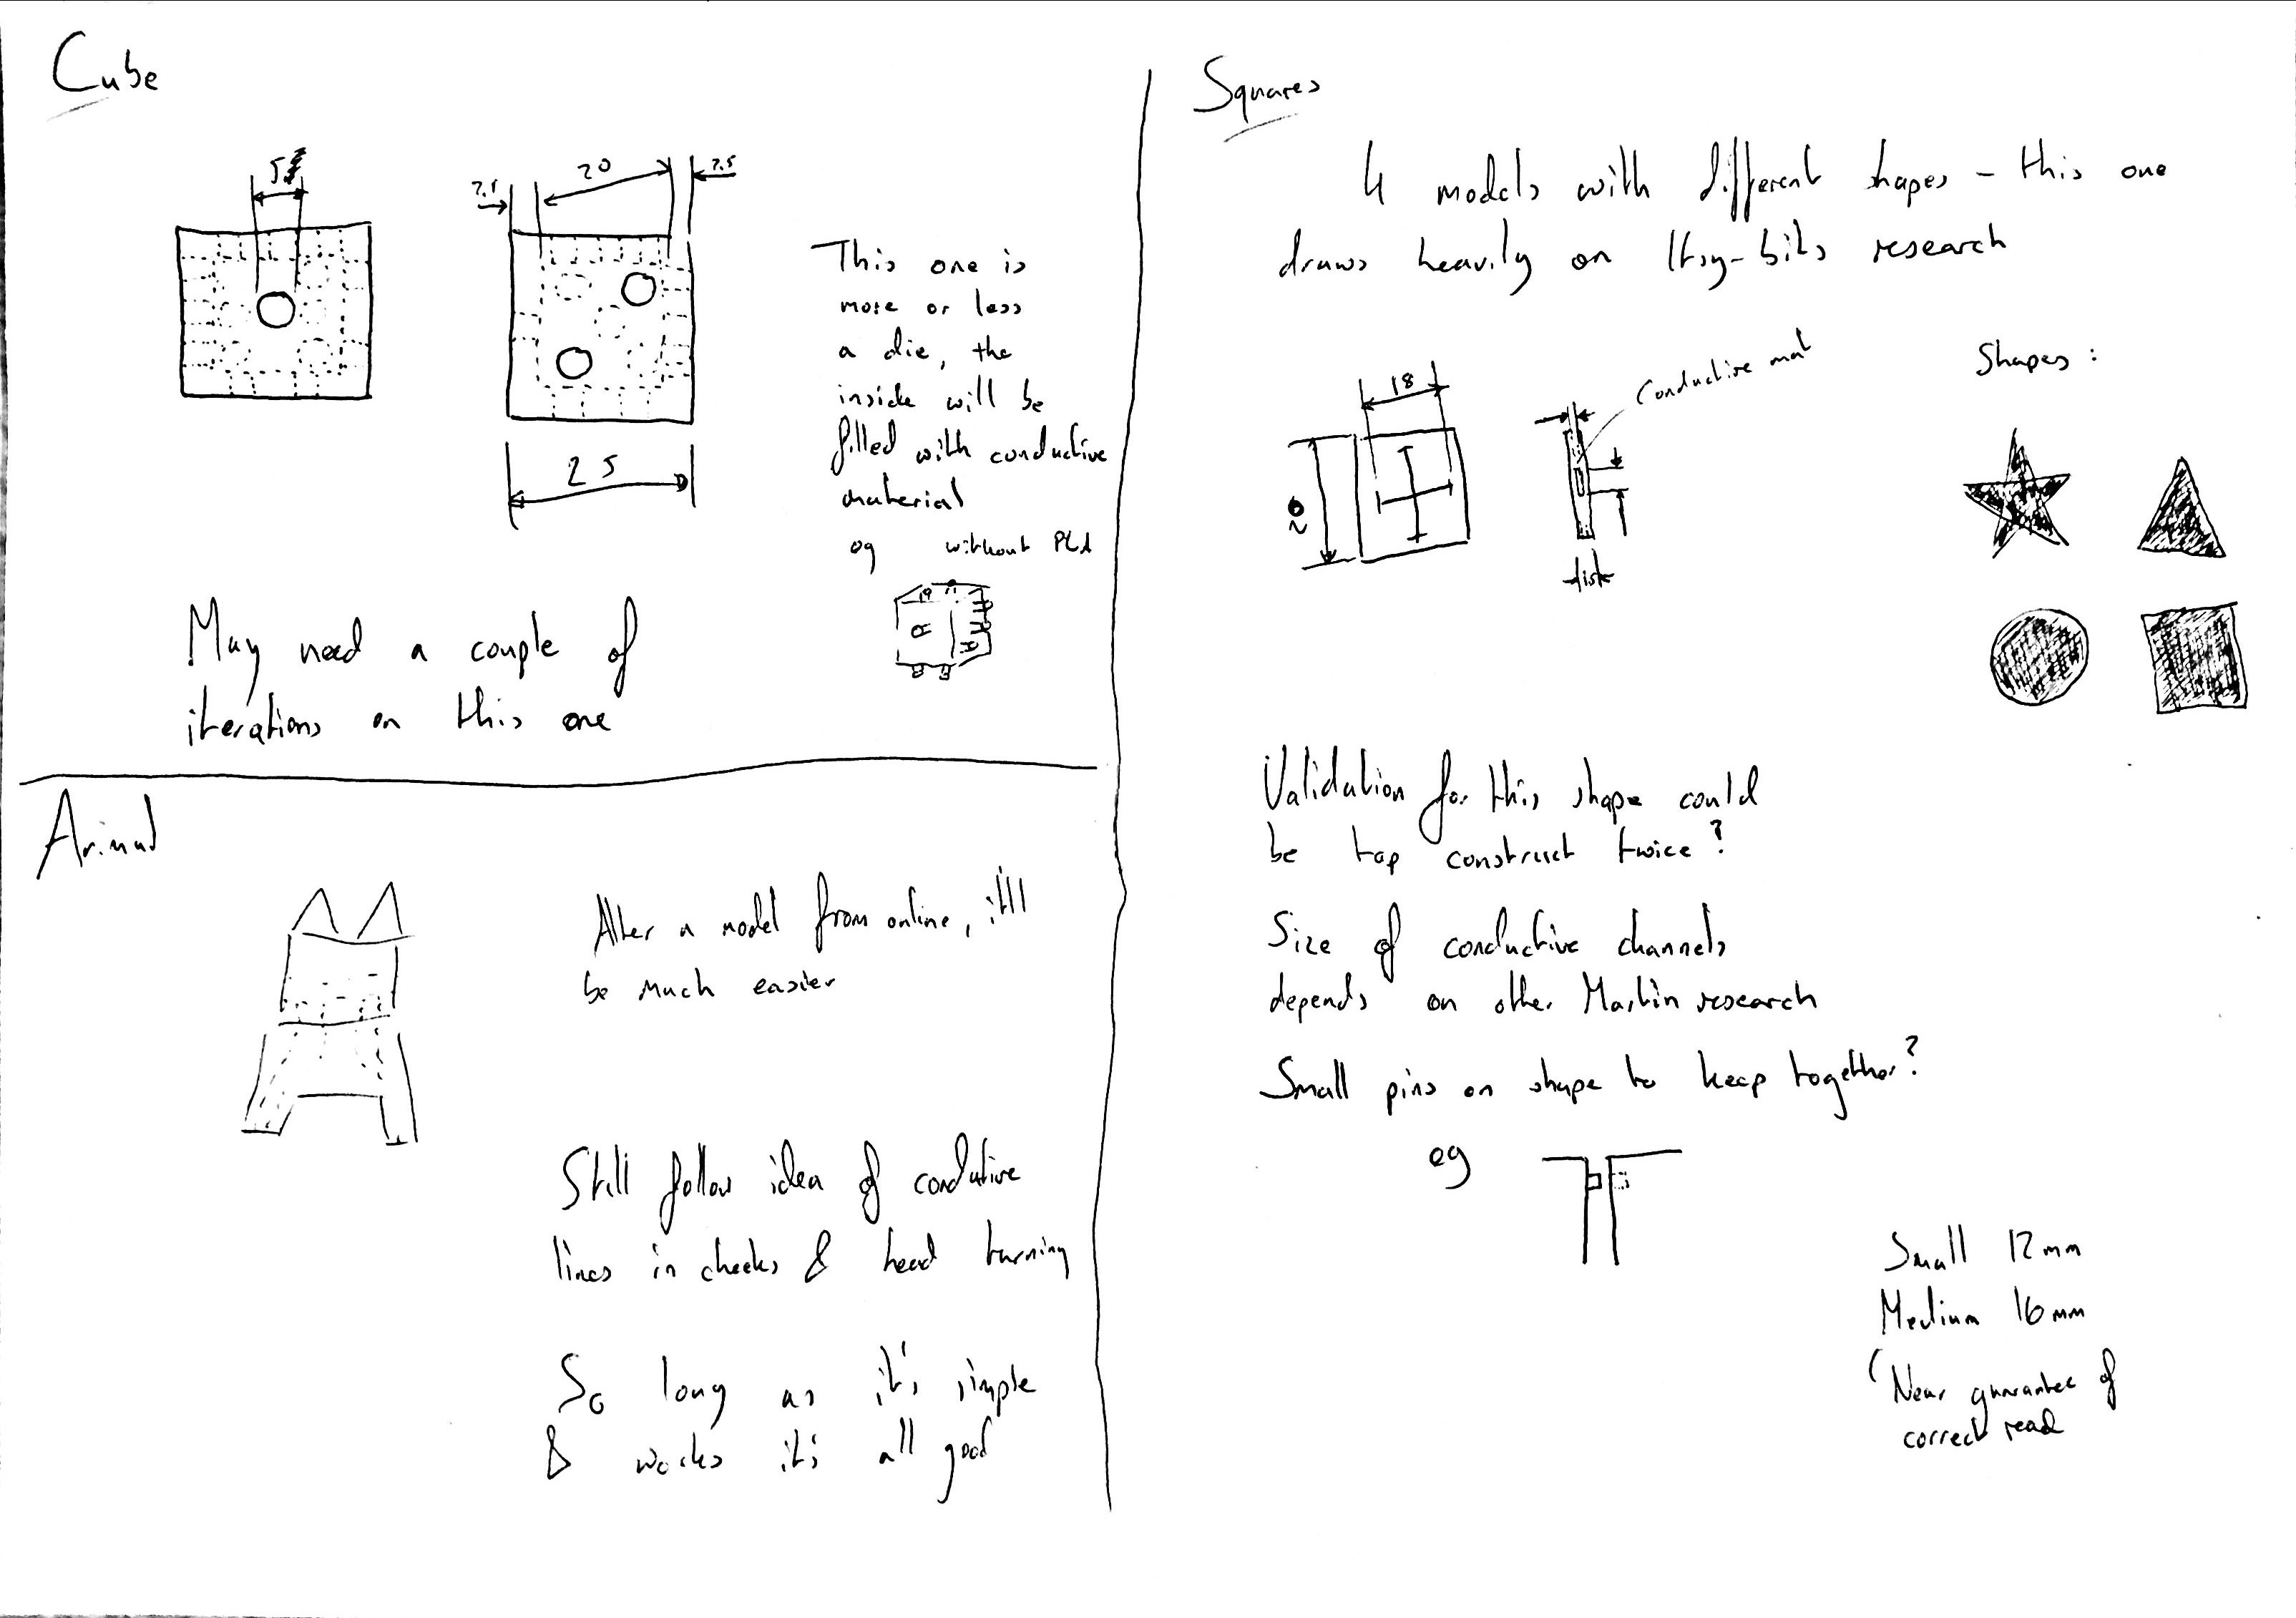
\includegraphics[width=\linewidth]{Appendices/prod_2.jpg}
    \caption{Initial production drawings for cube, animal and squares models}
    \label{fig:prod2}
\end{figure}

\begin{figure}
    \centering
    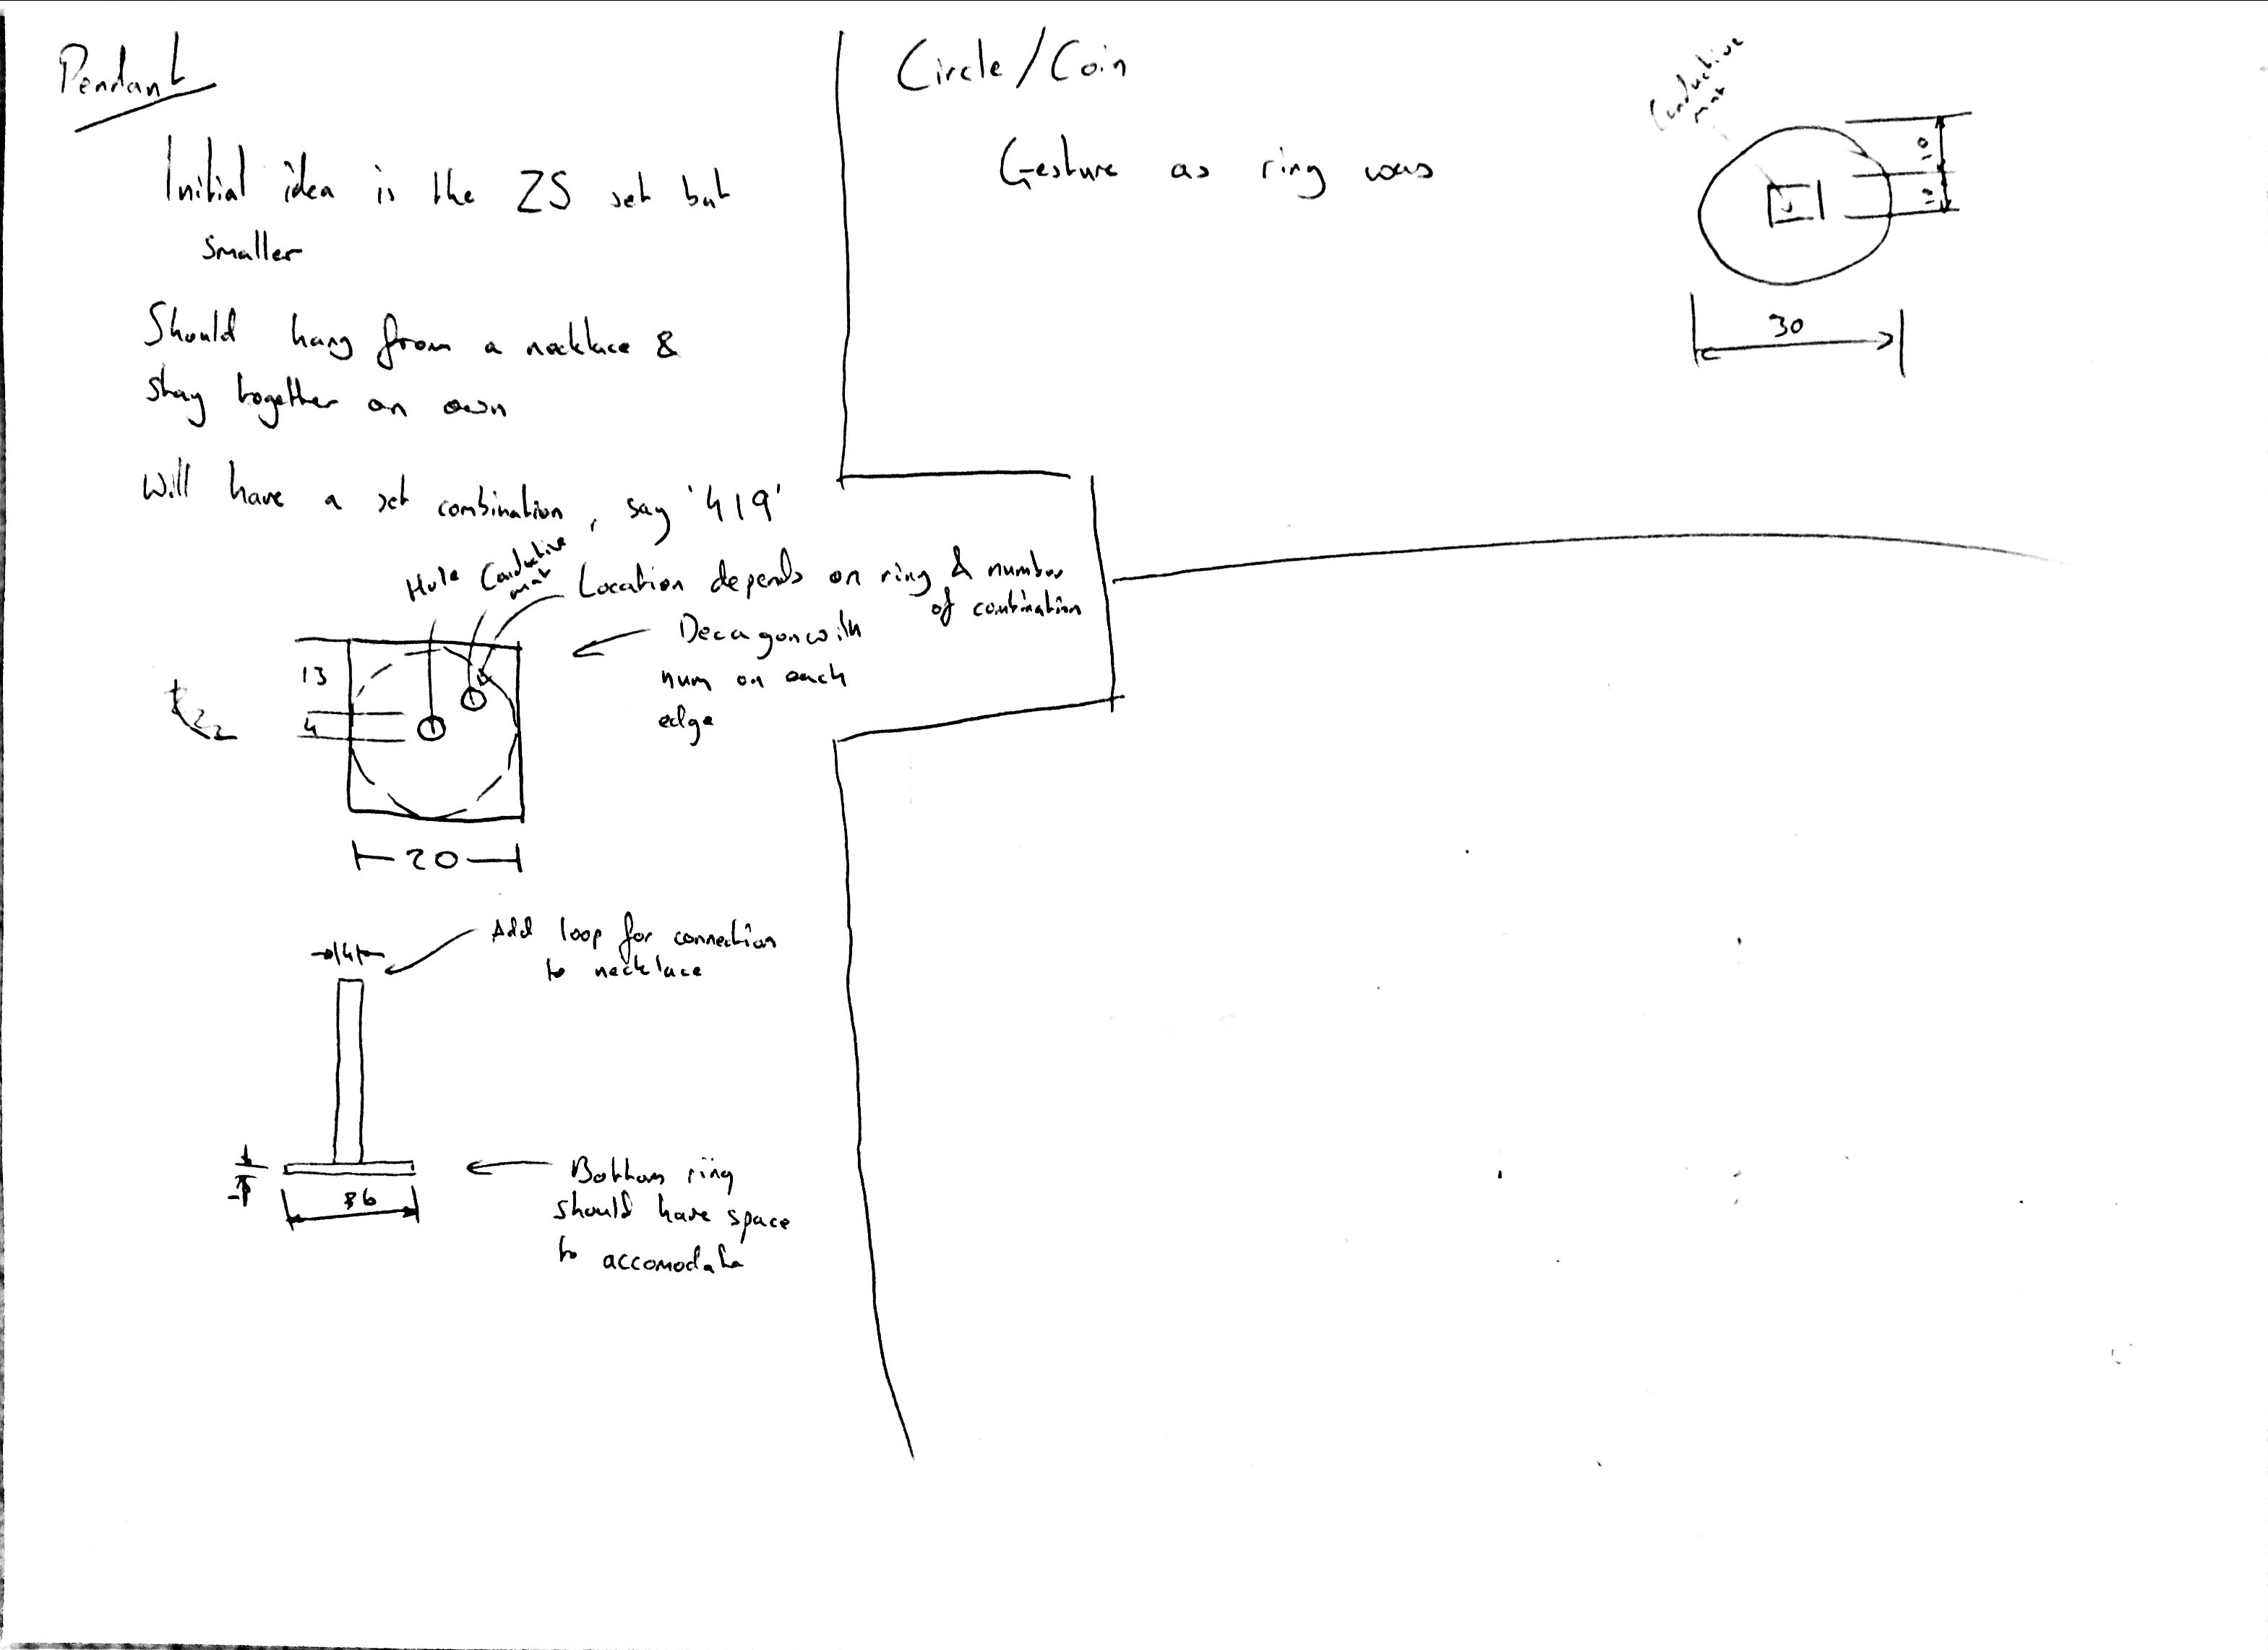
\includegraphics[width=\linewidth]{Appendices/prod_3.jpg}
    \caption{Initial production drawings for pendant and circle/coin models}
    \label{fig:prod3}
\end{figure}
\clearpage

\chapter{Model Interaction Instructions}
\label{sec:instructions}

The full sheet of interaction instructions given to participants can be found in Figures \ref{fig:interaction1}, \ref{fig:interaction2} and \ref{fig:interaction3}.

\begin{figure}
    \centering
    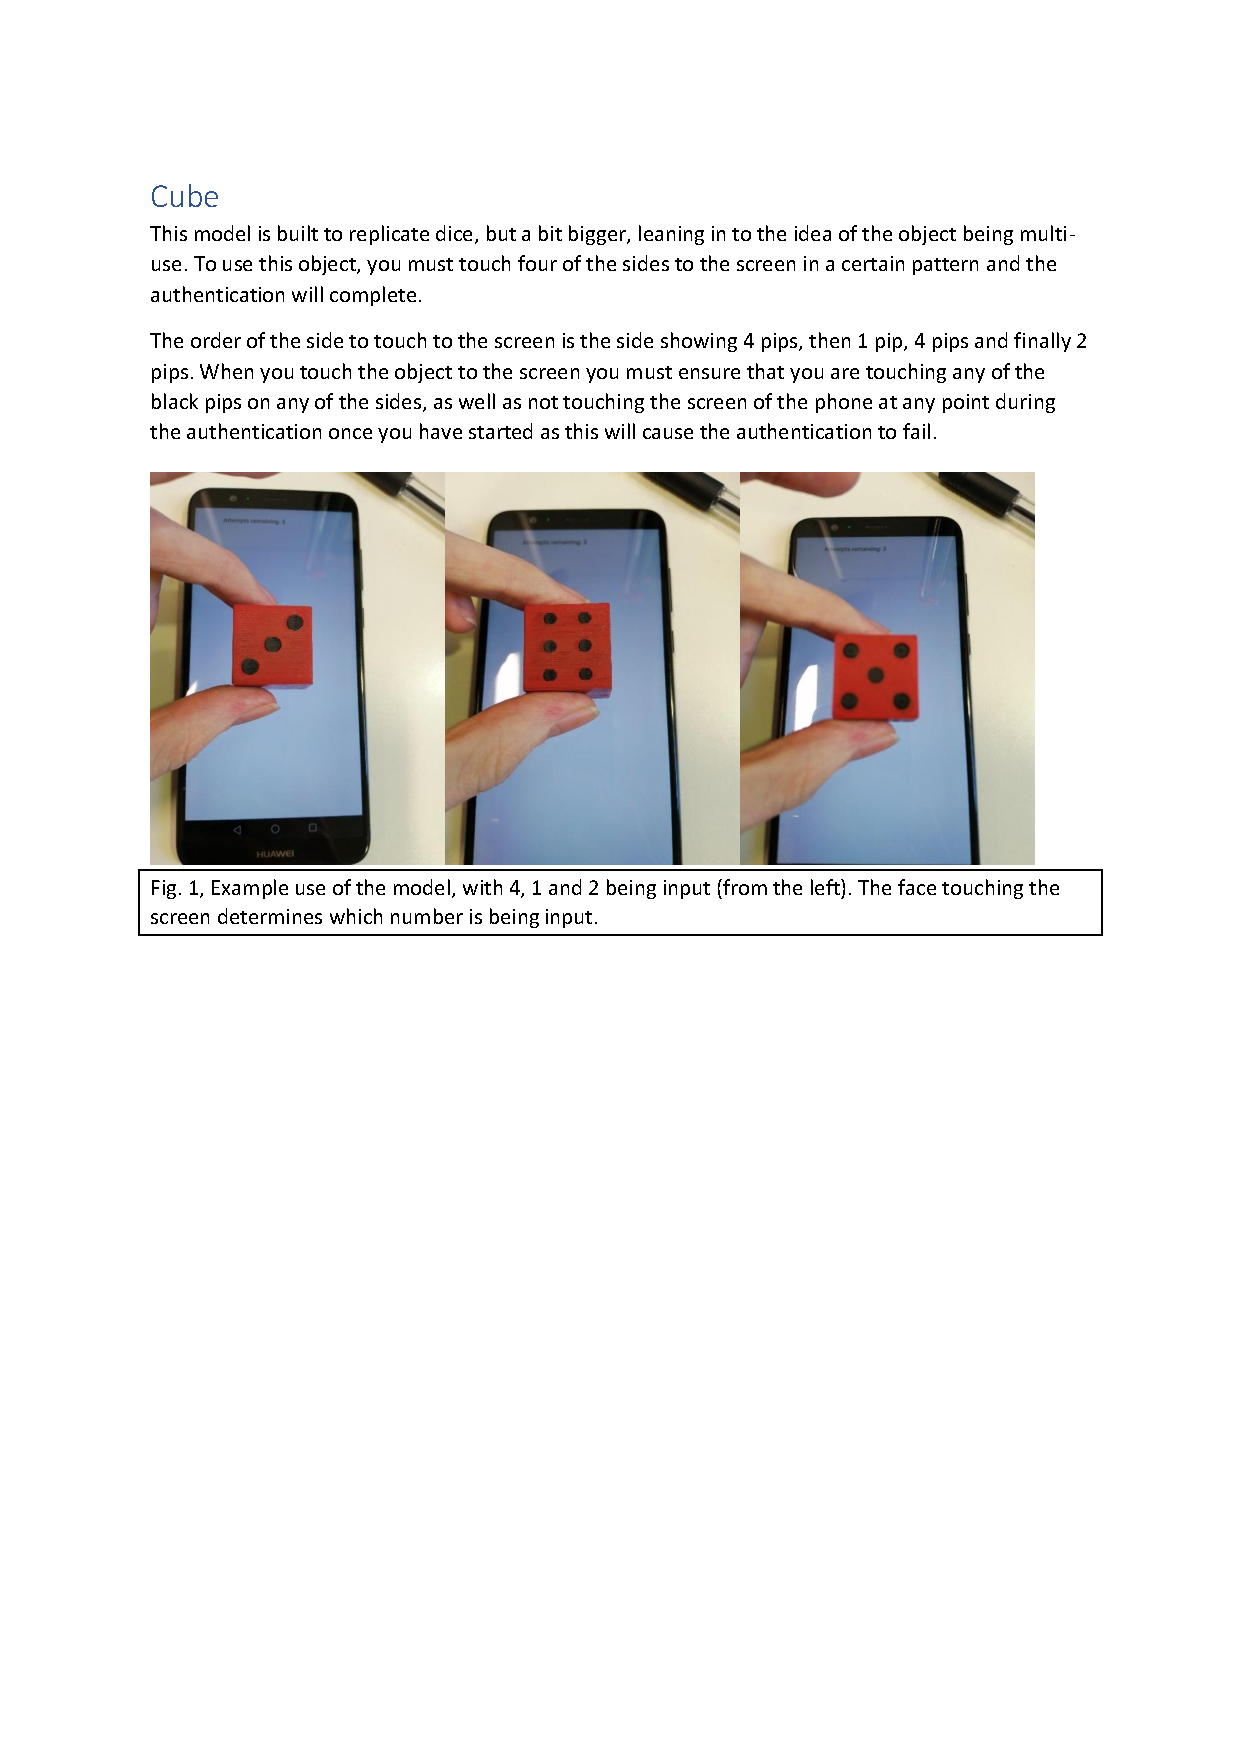
\includegraphics[page=1,width=\linewidth]{Appendices/Model Instructions.pdf}
    \caption{Model instructions issued to participants during the initial meeting to familiarise with assigned model. (part 1/3)}
    \label{fig:interaction1}
\end{figure}


\begin{figure}
    \centering
    \includegraphics[page=2,width=\linewidth]{Appendices/Model Instructions.pdf}
    \caption{Model instructions issued to participants during the initial meeting to familiarise with assigned model. (part 2/3)}
    \label{fig:interaction2}
\end{figure}

\begin{figure}
    \centering
    \includegraphics[page=3,width=\linewidth]{Appendices/Model Instructions.pdf}
    \caption{Model instructions issued to participants during the initial meeting to familiarise with assigned model. (part 3/3)}
    \label{fig:interaction3}
\end{figure}

\newpage

\chapter{Initial Interview Survey}
\label{sec:demo}
In this section, the questions from the survey given in the initial meeting with each participant are specified. For part one, selection questions are specified with the complete list of options given. For part two, these questions all follow the same pattern of selection questions with the choice of one of the following: Completely Disagree, Largely Disagree, Slightly Disagree, Slightly Agree, Largely Agree, Completely Agree.
\begin{itemize}
    \item Part 1 - Demographics
    \begin{itemize}
        \item Please enter the ID number you have been assigned. \textit{(Number input)}

        \item What is your age? \textit{(Selection, one of: Under 21, 21-25, 26-30, 31-35, 36-40, 41-45, 46-50, Over 50)}

        \item Please select your gender: \textit{(Selection, one of: Male, Female, Prefer not to say, Prefer to self-describe).} If 'Prefer to self-describe':

        \item Prefer to self describe. \textit{(Open answer)}

        \item What is your country of residence? \textit{(Open answer)}

        \item Please select your professional status: \textit{(Selection, one of: Student, Employed, Unemployed, Other)}

        \item Are you currently working from home? \textit{(Selection, one of: Yes, No)}

        \item Are you familiar with other methods of two-factor authentication? \textit{(Selection, one of: Yes, No)}
    \end{itemize}
    \item Part 2 - ATI Scale
    \begin{itemize}
        \item I like to occupy myself in greater detail with technical systems.

        \item I like testing the functions of new technical systems.
        
        \item I predominantly deal with technical systems because I have to.
        
        \item When I have a new technical system in from of me, I try it out intensively.
        
        \item I enjoy spending time becoming acquainted with a new technical system.
        
        \item It is enough for me that a technical system works; I don't care how or why.
        
        \item I try to understand how a technical system exactly works.
        
        \item It is enough for me to know the basic functions of a technical system.
        
        \item I try to make full use of the capabilities of a technical system.
    \end{itemize}
\end{itemize}

\chapter{Exit Interview Survey}
\label{sec:interview}
In this section, questions given during the final meeting in the study with each participant are specified. For part one, selection questions are specified with the complete list of options given. For part two, these questions all follow the same pattern of selection questions with a choice of one of the following: Strongly Agree, Agree, Neither Agree nor Disagree, Disagree, Strongly Disagree.
\begin{itemize}
    \item Part 1 - Model information
    \begin{itemize}
        \item Please enter the ID number you have been assigned
        \item Which model were you tasked with using? \textit{(Selection, one of: Credit Card, Pendant, Cube)}
        \item Did the model break or otherwise stop functioning during the study? \textit{(Selection, one of: Yes, No)}
    \end{itemize}
    \item Part 2 - System usability scale
    \begin{itemize}
        \item I would like to use this type of authentication frequently
        \item Using the model was needlessly complex.
        \item Using the model was easy
        \item Using the model would require some support from an experienced person
        \item The object was well integrated into daily life (ie, it was not jarring to use the object when needed)
        \item The object was too inconsistent
        \item It would be easy to learn how to use the model for authentication
        \item Using the model as authentication was very cumbersome
        \item You feel confident you know how to use the model to authenticate
        \item There was a lot to learn before you could use the model for authentication
    \end{itemize}
\end{itemize}

\chapter{Exit Interview and Codebook}

In this section, the questions given during the exit interview are first specified, with the developed codebook used for the analysis of the meeting transcripts following, along with the number of occurrences for each code.

\begin{itemize}
    \item Part 1 - Experience in the past week
    \begin{itemize}
        \item How was interacting with the object in the past week?
        \begin{itemize}
            \item Was there anything in particular that you like or disliked?
        \end{itemize}
        \item Was there anything that went wrong?
        \item Was there anything that prevented you from using the item?
        \item What do you think of the shape and size of the item?
        \item If the item was a commercial product, would you consider buying it?
        \begin{itemize}
            \item If so, why? If not, why not?
        \end{itemize}
    \end{itemize}
    \item Part 2 - 2-factor authentication generally
    \begin{itemize}
        \item Are you familiar with using other 2-factor authentication methods, for example, for your banking or other services?
        \begin{itemize}
            \item If so, which ones? If not, why?
        \end{itemize}
        \item Would you prefer to use this method over other 2-factor authentication methods?
        \begin{itemize}
            \item If so, why? If not, why not and what could be changed to make it more attractive for use?
        \end{itemize}
        \item How secure does it feel to use the provided item for authentication?
        \begin{itemize}
            \item Is it more, less or about the same as other methods you have used?
        \end{itemize}
        \item For which kinds of services would you consider using this type of authentication in your daily life?
        \begin{itemize}
            \item Why those ones and not others?
        \end{itemize}
        \item For which devices would you consider using this type of authentication on?
        \begin{itemize}
            \item Why those and not others?
        \end{itemize}
    \end{itemize}
    \item Part 3 - Other models and 3D printing
    \begin{itemize}
        \item Having had the chance to use all 3 objects, which do you think you would prefer to use?
        \begin{itemize}
            \item Why? Were there things you liked more about the other objects than the one you were assigned?
        \end{itemize}
        \item Would you ever consider owning a 3D printer?
    \end{itemize}
    
\end{itemize}

\begin{table*}[]
\centering
 \resizebox{\textwidth}{!}{
    \begin{tabular}{p{2.5cm}|p{4cm}|p{9cm}|c}
        \toprule
        \textbf{Category} & \textbf{Code} & \textbf{Description} & \textbf{\#} \\
        \midrule
        Security & familiar\_2fa & Participant familiar with two-factor authentication & 3 \\
        & unsure & Unsure about the security of the models & 2 \\
        & secure & Feels the models are secure & 1 \\
        & safe & Feels the models are unlikely to be stolen & 2 \\
        & shoulder\_surfing & Feels vulnerable to shoulder surfing when using the models & 1 \\
        & requirement & Uses two factor authentication only when required to & 2 \\
        & no\_data & Feels they have nothing important to secure/nothing worth stealing & 1\\
        \midrule
        Usability & lacked\_feedback & Lacking in feedback when using the models & 2 \\
        & unique & Unique and novel method of authentication & 1 \\
        & learning\_curve & Felt there was a learning curve to using the models & 2 \\
        & disliked\_handheld\_use & Disliked using the models when away from a flat surface & 3 \\
        & portable & Felt the model was easy to carry around & 3 \\
        & forgettable & Felt the model was easy to forget to bring & 1 \\
        & inconsistent & Thought the interaction felt stilted or inconsistent & 3 \\
        & easy\_to\_use & Felt the interactions weren't any harder to use than other two factor authentication methods & 2 \\
        & preferred & Preferred to use the method over other 2FA methods & 3\\
        & slide & Models tended to slide on the phone screen & 3 \\
        & fragile & Models felt fragile & 2 \\
        & card\_favourite & Credit card model was their favourite to use & 2 \\
        & cube\_favourite & Cube model was their favourite & 1 \\
        & familiar & Familiarity of interaction method was important & 2 \\
        & enjoy & Enjoyment to use was important & 3 \\
        & card\_liked & Liked interactions with the credit card model &2 \\
        & pendant\_liked & Liked interactions with the pendant models & 2 \\
        & cube\_likes & Liked interactions with the cube model & 3 \\
        & future\_use & Would consider using in the future & 3 \\
        \midrule
        Method of use & tabletop\_only & Used only on tabletops during the study & 2 \\
        & banking & Would use for banking and other places 2fa already used for & 3 \\
        & single\_model & Would want to use one model for multiple services & 1 \\
        & any\_device & Would use on any device & 2 \\
        & stationary\_device & Would prefer to use on home computer/laptop only & 1 \\
        & home\_use & Would only use at home & 2 \\
        & global\_use & Would use anywhere & 1 \\
        \midrule
        3D Printing & would\_own & Would consider owning a 3D printer & 2 \\
        & not\_considering & Not currently thinking about owning a 3D printer & 1 \\
        & no\_adoption & Doesn't think there will be widespread adoption of 3D printers & 2 \\
        & adoption & Thinks there will be widespread adoption of 3D printers & 1 \\
        & copy\_shop & Anticipates 3D printing 'copy shop' types of businesses in the future & 2 \\
        Commercial & would\_not\_buy & Would be hesitant to buy any of the models in the future & 2 \\
        & would\_buy & Would buy in the future & 1 \\
        \midrule
        Improvement & improvement & Suggested improvement & 3 \\
        \bottomrule
    \end{tabular}}
    \caption{Codebook used for analysis of exit interviews.}
\end{table*}

\end{appendices}

%==================================================================================================================================
%   BIBLIOGRAPHY   

% The bibliography style is abbrvnat
% The bibliography always appears last, after the appendices.

\bibliographystyle{abbrvnat}

\bibliography{l4proj}

\end{document}
